\documentclass[10pt,sigconf,dvipsnames]{acmart}
\settopmatter{authorsperrow=4}

\usepackage{booktabs} % For formal tables

%\usepackage{etoolbox}
%\apptocmd{\thebibliography}{\scriptsize}{}{}

%\usepackage{etoolbox}
%\apptocmd{\thebibliography}{\scriptsize}{}{}
\usepackage{multirow}
%\usepackage{graphicx}
\usepackage{balance}  % for  \balance command ON LAST PAGE  (only there!)

\usepackage{color}
\usepackage{xcolor}
\usepackage{amssymb}% http://ctan.org/pkg/amssymb
\usepackage{pifont}% http://ctan.org/pkg/pifont

\usepackage{pifont}
\usepackage{url}

\usepackage{booktabs} % For formal tables

\usepackage{enumitem}
\usepackage{amsmath}
%\usepackage[linesnumbered,ruled]{algorithm2e}
\usepackage[linesnumbered,ruled,vlined]{algorithm2e}


\usepackage{graphicx}
\usepackage[font=scriptsize]{subfig}
\usepackage[font=small,labelfont=bf]{caption}
%\usepackage{subfigure}
\usepackage{epsfig}

% For statistical figure
\usepackage{tikz}
\usetikzlibrary{snakes}

\newcommand{\colorForRevisions}{red}
\newcommand{\gram}[1]{\textcolor{green}{\bf [Grammarly: #1]}}

\DeclareMathOperator*{\argmax}{arg\,max\:}
\DeclareMathOperator*{\argmin}{arg\,min\:}

%\newcommand\inv[1]{#1\raisebox{1.15ex}{$\scriptscriptstyle-\!1$}}
\newcommand{\invone}{^{\raisebox{.2ex}{$\scriptscriptstyle-1$}}}
\newcommand{\invhalf}{^{\raisebox{.2ex}{$\scriptscriptstyle-0.5$}}}


\def\SPSB#1#2{\rlap{\textsuperscript{{#1}}}\SB{#2}}
\def\SP#1{\textsuperscript{{#1}}}
\def\SB#1{\textsubscript{{#1}}}



\copyrightyear{2020}
\acmYear{2020}
\setcopyright{acmcopyright}\acmConference[SIGMOD'20]{Proceedings of the 2020 ACM SIGMOD International Conference on Management of Data}{June 14--19, 2020}{Portland, OR, USA}
\acmBooktitle{Proceedings of the 2020 ACM SIGMOD International Conference on Management of Data (SIGMOD'20), June 14--19, 2020, Portland, OR, USA}
\acmPrice{15.00}
\acmDOI{10.1145/3318464.3389760}
\acmISBN{978-1-4503-6735-6/20/06}

\settopmatter{printacmref=true}

% Copyright
%\setcopyright{none}
%\setcopyright{acmcopyright}
%\setcopyright{acmlicensed}
\setcopyright{rightsretained}
%\setcopyright{usgov}
%\setcopyright{usgovmixed}
%\setcopyright{cagov}
%\setcopyright{cagovmixed}

% DOI
%\acmDOI{10.475/123_4}

% ISBN
%\acmISBN{123-4567-24-567/08/06}

%Conference
%\acmConference[SIGMOD'20]{ACM SIGMOD conference}{June 2020}{Portland, OR, USA}
%\acmYear{2020}
%\copyrightyear{2020}


%\acmArticle{4}
%\acmPrice{15.00}

% These commands are optional
%\acmBooktitle{Transactions of the ACM Woodstock conference}
%\editor{Jennifer B. Sartor}
%\editor{Theo D'Hondt}
%\editor{Wolfgang De Meuter}


\settopmatter{printacmref=true}
% THIS COMMAND WILL SHRINK PAPER BY 2% BY REMOVING UNNEEDED SPACES!
%\renewcommand{\baselinestretch}{0.94}



\begin{document}
\fancyhead{}


\title{Debunking Four Long-Standing Misconceptions \\ of Time-Series Distance Measures}
%\titlenote{Produces the permission block, and
%  copyright information}
%\subtitle{Extended Abstract}
%\subtitlenote{The full version of the author's guide is available as
%  \texttt{acmart.pdf} document}


\author{John Paparrizos}
%\authornote{Dr.~Trovato insisted his name be first.}
%\orcid{1234-5678-9012}
\affiliation{%
  \institution{University of Chicago\\ \small{jopa@uchicago.edu}}
%  \streetaddress{jopa@uchicago.edu}
%  \city{Dublin}
%  \state{Ohio}
%  \postcode{43017-6221}
}
%\email{jopa@uchicago.edu}

\author{Chunwei Liu}
%\authornote{Dr.~Trovato insisted his name be first.}
%\orcid{1234-5678-9012}

\affiliation{%
  \institution{University of Chicago\\ \small{chunwei@uchicago.edu}}
%  \streetaddress{P.O. Box 1212}
%  \city{Dublin}
%  \state{Ohio}
%  \postcode{43017-6221}
}
%\email{chunwei@uchicago.edu}

\author{Aaron J. Elmore}
%\authornote{Dr.~Trovato insisted his name be first.}
%\orcid{1234-5678-9012}
\affiliation{%
  \institution{University of Chicago\\ \small{aelmore@uchicago.edu}}
% \streetaddress{P.O. Box 1212}
%  \city{Dublin}
%  \state{Ohio}
%  \postcode{43017-6221}
}
%\email{aelmore@uchicago.edu}

\author{Michael J. Franklin}
%\authornote{Dr.~Trovato insisted his name be first.}
%\orcid{1234-5678-9012}
\affiliation{%
  \institution{University of Chicago\\ \small{mjfranklin@uchicago.edu}}
%  \streetaddress{P.O. Box 1212}
%  \city{Dublin}
%  \state{Ohio}
%  \postcode{43017-6221}
}
%\email{mjfranklin@uchicago.edu}


% The default list of authors is too long for headers.
%\renewcommand{\shortauthors}{B. Trovato et al.}


\begin{abstract}
%In a multitude of scientific and industrial applications, the basis for most data analyses involves the querying of time-series. 
Distance measures are core building blocks in time-series analysis and the subject of active research for decades. Unfortunately, the most detailed experimental study in this area is outdated (over a decade old) and, naturally, does not reflect recent progress. Importantly, this study (i) omitted multiple distance measures, including a classic measure in the time-series literature; (ii) considered only a single time-series normalization method; and (iii) reported only raw classification error rates without statistically validating the findings, resulting in or fueling four misconceptions in the time-series literature. Motivated by the aforementioned drawbacks and our curiosity to shed some light on these misconceptions, we comprehensively evaluate \textcolor{black}{$71$} time-series distance measures. Specifically, our study includes (i) $8$ normalization methods; (ii) $52$ lock-step measures; (iii) $4$ sliding measures; (iv) $7$ elastic measures; \textcolor{black}{(v) $4$ kernel functions; and (vi) $4$ embedding measures}. We extensively evaluate these measures across $128$ time-series datasets using rigorous statistical analysis. Our findings debunk four long-standing misconceptions that significantly alter the landscape of what is known about existing distance measures. With the new foundations in place, we discuss open challenges and promising directions.
\end{abstract}

%
% The code below should be generated by the tool at
% http://dl.acm.org/ccs.cfm
% Please copy and paste the code instead of the example below.
%
%\begin{CCSXML}
%<ccs2012>
% <concept>
%  <concept_id>10010520.10010553.10010562</concept_id>
%  <concept_desc>Computer systems organization~Embedded systems</concept_desc>
%  <concept_significance>500</concept_significance>
% </concept>
% <concept>
%  <concept_id>10010520.10010575.10010755</concept_id>
%  <concept_desc>Computer systems organization~Redundancy</concept_desc>
%  <concept_significance>300</concept_significance>
% </concept>
% <concept>
%  <concept_id>10010520.10010553.10010554</concept_id>
%  <concept_desc>Computer systems organization~Robotics</concept_desc>
%  <concept_significance>100</concept_significance>
% </concept>
% <concept>
%  <concept_id>10003033.10003083.10003095</concept_id>
%  <concept_desc>Networks~Network reliability</concept_desc>
%  <concept_significance>100</concept_significance>
% </concept>
%</ccs2012>
%\end{CCSXML}

%\ccsdesc[500]{Computer systems organization~Embedded systems}
%\ccsdesc[300]{Computer systems organization~Redundancy}
%\ccsdesc{Computer systems organization~Robotics}
%\ccsdesc[100]{Networks~Network reliability}

%\keywords{ACM proceedings, \LaTeX, text tagging}

\maketitle

%\section{Introduction}

The \textit{proceedings} are the records of a conference.\footnote{This
  is a footnote}  ACM seeks
to give these conference by-products a uniform, high-quality
appearance.  To do this, ACM has some rigid requirements for the
format of the proceedings documents: there is a specified format
(balanced double columns), a specified set of fonts (Arial or
Helvetica and Times Roman) in certain specified sizes, a specified
live area, centered on the page, specified size of margins, specified
column width and gutter size.

\section{The Body of The Paper}
Typically, the body of a paper is organized into a hierarchical
structure, with numbered or unnumbered headings for sections,
subsections, sub-subsections, and even smaller sections.  The command
\texttt{{\char'134}section} that precedes this paragraph is part of
such a hierarchy.\footnote{This is a footnote.} \LaTeX\ handles the
numbering and placement of these headings for you, when you use the
appropriate heading commands around the titles of the headings.  If
you want a sub-subsection or smaller part to be unnumbered in your
output, simply append an asterisk to the command name.  Examples of
both numbered and unnumbered headings will appear throughout the
balance of this sample document.

Because the entire article is contained in the \textbf{document}
environment, you can indicate the start of a new paragraph with a
blank line in your input file; that is why this sentence forms a
separate paragraph.

\subsection{Type Changes and {\itshape Special} Characters}

We have already seen several typeface changes in this sample.  You can
indicate italicized words or phrases in your text with the command
\texttt{{\char'134}textit}; emboldening with the command
\texttt{{\char'134}textbf} and typewriter-style (for instance, for
computer code) with \texttt{{\char'134}texttt}.  But remember, you do
not have to indicate typestyle changes when such changes are part of
the \textit{structural} elements of your article; for instance, the
heading of this subsection will be in a sans serif\footnote{Another
  footnote here.  Let's make this a rather long one to see how it
  looks.} typeface, but that is handled by the document class file.
Take care with the use of\footnote{Another footnote.}  the
curly braces in typeface changes; they mark the beginning and end of
the text that is to be in the different typeface.

You can use whatever symbols, accented characters, or non-English
characters you need anywhere in your document; you can find a complete
list of what is available in the \textit{\LaTeX\ User's Guide}
\cite{Lamport:LaTeX}.

\subsection{Math Equations}
You may want to display math equations in three distinct styles:
inline, numbered or non-numbered display.  Each of
the three are discussed in the next sections.

\subsubsection{Inline (In-text) Equations}
A formula that appears in the running text is called an
inline or in-text formula.  It is produced by the
\textbf{math} environment, which can be
invoked with the usual \texttt{{\char'134}begin\,\ldots{\char'134}end}
construction or with the short form \texttt{\$\,\ldots\$}. You
can use any of the symbols and structures,
from $\alpha$ to $\omega$, available in
\LaTeX~\cite{Lamport:LaTeX}; this section will simply show a
few examples of in-text equations in context. Notice how
this equation:
\begin{math}
  \lim_{n\rightarrow \infty}x=0
\end{math},
set here in in-line math style, looks slightly different when
set in display style.  (See next section).

\subsubsection{Display Equations}
A numbered display equation---one set off by vertical space from the
text and centered horizontally---is produced by the \textbf{equation}
environment. An unnumbered display equation is produced by the
\textbf{displaymath} environment.

Again, in either environment, you can use any of the symbols
and structures available in \LaTeX\@; this section will just
give a couple of examples of display equations in context.
First, consider the equation, shown as an inline equation above:
\begin{equation}
  \lim_{n\rightarrow \infty}x=0
\end{equation}
Notice how it is formatted somewhat differently in
the \textbf{displaymath}
environment.  Now, we'll enter an unnumbered equation:
\begin{displaymath}
  \sum_{i=0}^{\infty} x + 1
\end{displaymath}
and follow it with another numbered equation:
\begin{equation}
  \sum_{i=0}^{\infty}x_i=\int_{0}^{\pi+2} f
\end{equation}
just to demonstrate \LaTeX's able handling of numbering.

\subsection{Citations}
Citations to articles~\cite{bowman:reasoning,
clark:pct, braams:babel, herlihy:methodology},
conference proceedings~\cite{clark:pct} or maybe
books \cite{Lamport:LaTeX, salas:calculus} listed
in the Bibliography section of your
article will occur throughout the text of your article.
You should use BibTeX to automatically produce this bibliography;
you simply need to insert one of several citation commands with
a key of the item cited in the proper location in
the \texttt{.tex} file~\cite{Lamport:LaTeX}.
The key is a short reference you invent to uniquely
identify each work; in this sample document, the key is
the first author's surname and a
word from the title.  This identifying key is included
with each item in the \texttt{.bib} file for your article.

The details of the construction of the \texttt{.bib} file
are beyond the scope of this sample document, but more
information can be found in the \textit{Author's Guide},
and exhaustive details in the \textit{\LaTeX\ User's
Guide} by Lamport~\shortcite{Lamport:LaTeX}.

This article shows only the plainest form
of the citation command, using \texttt{{\char'134}cite}.

Some examples.  A paginated journal article \cite{Abril07}, an enumerated
journal article \cite{Cohen07}, a reference to an entire issue \cite{JCohen96},
a monograph (whole book) \cite{Kosiur01}, a monograph/whole book in a series (see 2a in spec. document)
\cite{Harel79}, a divisible-book such as an anthology or compilation \cite{Editor00}
followed by the same example, however we only output the series if the volume number is given
\cite{Editor00a} (so Editor00a's series should NOT be present since it has no vol. no.),
a chapter in a divisible book \cite{Spector90}, a chapter in a divisible book
in a series \cite{Douglass98}, a multi-volume work as book \cite{Knuth97},
an article in a proceedings (of a conference, symposium, workshop for example)
(paginated proceedings article) \cite{Andler79}, a proceedings article
with all possible elements \cite{Smith10}, an example of an enumerated
proceedings article \cite{VanGundy07},
an informally published work \cite{Harel78}, a doctoral dissertation \cite{Clarkson85},
a master's thesis: \cite{anisi03}, an online document / world wide web
resource \cite{Thornburg01, Ablamowicz07, Poker06}, a video game (Case 1) \cite{Obama08} and (Case 2) \cite{Novak03}
and \cite{Lee05} and (Case 3) a patent \cite{JoeScientist001},
work accepted for publication \cite{rous08}, 'YYYYb'-test for prolific author
\cite{SaeediMEJ10} and \cite{SaeediJETC10}. Other cites might contain
'duplicate' DOI and URLs (some SIAM articles) \cite{Kirschmer:2010:AEI:1958016.1958018}.
Boris / Barbara Beeton: multi-volume works as books
\cite{MR781536} and \cite{MR781537}.

A couple of citations with DOIs: \cite{2004:ITE:1009386.1010128,
  Kirschmer:2010:AEI:1958016.1958018}.

Online citations: \cite{TUGInstmem, Thornburg01, CTANacmart}.


\subsection{Tables}
Because tables cannot be split across pages, the best
placement for them is typically the top of the page
nearest their initial cite.  To
ensure this proper ``floating'' placement of tables, use the
environment \textbf{table} to enclose the table's contents and
the table caption.  The contents of the table itself must go
in the \textbf{tabular} environment, to
be aligned properly in rows and columns, with the desired
horizontal and vertical rules.  Again, detailed instructions
on \textbf{tabular} material
are found in the \textit{\LaTeX\ User's Guide}.

Immediately following this sentence is the point at which
Table~\ref{tab:freq} is included in the input file; compare the
placement of the table here with the table in the printed
output of this document.

\begin{table}
  \caption{Frequency of Special Characters}
  \label{tab:freq}
  \begin{tabular}{ccl}
    \toprule
    Non-English or Math&Frequency&Comments\\
    \midrule
    \O & 1 in 1,000& For Swedish names\\
    $\pi$ & 1 in 5& Common in math\\
    \$ & 4 in 5 & Used in business\\
    $\Psi^2_1$ & 1 in 40,000& Unexplained usage\\
  \bottomrule
\end{tabular}
\end{table}

To set a wider table, which takes up the whole width of the page's
live area, use the environment \textbf{table*} to enclose the table's
contents and the table caption.  As with a single-column table, this
wide table will ``float'' to a location deemed more desirable.
Immediately following this sentence is the point at which
Table~\ref{tab:commands} is included in the input file; again, it is
instructive to compare the placement of the table here with the table
in the printed output of this document.


\begin{table*}
  \caption{Some Typical Commands}
  \label{tab:commands}
  \begin{tabular}{ccl}
    \toprule
    Command &A Number & Comments\\
    \midrule
    \texttt{{\char'134}author} & 100& Author \\
    \texttt{{\char'134}table}& 300 & For tables\\
    \texttt{{\char'134}table*}& 400& For wider tables\\
    \bottomrule
  \end{tabular}
\end{table*}
% end the environment with {table*}, NOTE not {table}!

It is strongly recommended to use the package booktabs~\cite{Fear05}
and follow its main principles of typography with respect to tables:
\begin{enumerate}
\item Never, ever use vertical rules.
\item Never use double rules.
\end{enumerate}
It is also a good idea not to overuse horizontal rules.


\subsection{Figures}

Like tables, figures cannot be split across pages; the best placement
for them is typically the top or the bottom of the page nearest their
initial cite.  To ensure this proper ``floating'' placement of
figures, use the environment \textbf{figure} to enclose the figure and
its caption.

This sample document contains examples of \texttt{.eps} files to be
displayable with \LaTeX.  If you work with pdf\LaTeX, use files in the
\texttt{.pdf} format.  Note that most modern \TeX\ systems will convert
\texttt{.eps} to \texttt{.pdf} for you on the fly.  More details on
each of these are found in the \textit{Author's Guide}.

\begin{figure}
\includegraphics{fly}
\caption{A sample black and white graphic.}
\end{figure}

\begin{figure}
\includegraphics[height=1in, width=1in]{fly}
\caption{A sample black and white graphic
that has been resized with the \texttt{includegraphics} command.}
\end{figure}


As was the case with tables, you may want a figure that spans two
columns.  To do this, and still to ensure proper ``floating''
placement of tables, use the environment \textbf{figure*} to enclose
the figure and its caption.  And don't forget to end the environment
with \textbf{figure*}, not \textbf{figure}!

\begin{figure*}
\includegraphics{flies}
\caption{A sample black and white graphic
that needs to span two columns of text.}
\end{figure*}


\begin{figure}
\includegraphics[height=1in, width=1in]{rosette}
\caption{A sample black and white graphic that has
been resized with the \texttt{includegraphics} command.}
\end{figure}

\subsection{Theorem-like Constructs}

Other common constructs that may occur in your article are the forms
for logical constructs like theorems, axioms, corollaries and proofs.
ACM uses two types of these constructs:  theorem-like and
definition-like.

Here is a theorem:
\begin{theorem}
  Let $f$ be continuous on $[a,b]$.  If $G$ is
  an antiderivative for $f$ on $[a,b]$, then
  \begin{displaymath}
    \int^b_af(t)\,dt = G(b) - G(a).
  \end{displaymath}
\end{theorem}

Here is a definition:
\begin{definition}
  If $z$ is irrational, then by $e^z$ we mean the
  unique number that has
  logarithm $z$:
  \begin{displaymath}
    \log e^z = z.
  \end{displaymath}
\end{definition}

The pre-defined theorem-like constructs are \textbf{theorem},
\textbf{conjecture}, \textbf{proposition}, \textbf{lemma} and
\textbf{corollary}.  The pre-defined de\-fi\-ni\-ti\-on-like constructs are
\textbf{example} and \textbf{definition}.  You can add your own
constructs using the \textsl{amsthm} interface~\cite{Amsthm15}.  The
styles used in the \verb|\theoremstyle| command are \textbf{acmplain}
and \textbf{acmdefinition}.

Another construct is \textbf{proof}, for example,

\begin{proof}
  Suppose on the contrary there exists a real number $L$ such that
  \begin{displaymath}
    \lim_{x\rightarrow\infty} \frac{f(x)}{g(x)} = L.
  \end{displaymath}
  Then
  \begin{displaymath}
    l=\lim_{x\rightarrow c} f(x)
    = \lim_{x\rightarrow c}
    \left[ g{x} \cdot \frac{f(x)}{g(x)} \right ]
    = \lim_{x\rightarrow c} g(x) \cdot \lim_{x\rightarrow c}
    \frac{f(x)}{g(x)} = 0\cdot L = 0,
  \end{displaymath}
  which contradicts our assumption that $l\neq 0$.
\end{proof}

\section{Conclusions}
This paragraph will end the body of this sample document.
Remember that you might still have Acknowledgments or
Appendices; brief samples of these
follow.  There is still the Bibliography to deal with; and
we will make a disclaimer about that here: with the exception
of the reference to the \LaTeX\ book, the citations in
this paper are to articles which have nothing to
do with the present subject and are used as
examples only.
%\end{document}  % This is where a 'short' article might terminate



\appendix
%Appendix A
\section{Headings in Appendices}
The rules about hierarchical headings discussed above for
the body of the article are different in the appendices.
In the \textbf{appendix} environment, the command
\textbf{section} is used to
indicate the start of each Appendix, with alphabetic order
designation (i.e., the first is A, the second B, etc.) and
a title (if you include one).  So, if you need
hierarchical structure
\textit{within} an Appendix, start with \textbf{subsection} as the
highest level. Here is an outline of the body of this
document in Appendix-appropriate form:
\subsection{Introduction}
\subsection{The Body of the Paper}
\subsubsection{Type Changes and  Special Characters}
\subsubsection{Math Equations}
\paragraph{Inline (In-text) Equations}
\paragraph{Display Equations}
\subsubsection{Citations}
\subsubsection{Tables}
\subsubsection{Figures}
\subsubsection{Theorem-like Constructs}
\subsubsection*{A Caveat for the \TeX\ Expert}
\subsection{Conclusions}
\subsection{References}
Generated by bibtex from your \texttt{.bib} file.  Run latex,
then bibtex, then latex twice (to resolve references)
to create the \texttt{.bbl} file.  Insert that \texttt{.bbl}
file into the \texttt{.tex} source file and comment out
the command \texttt{{\char'134}thebibliography}.
% This next section command marks the start of
% Appendix B, and does not continue the present hierarchy
\section{More Help for the Hardy}

Of course, reading the source code is always useful.  The file
\path{acmart.pdf} contains both the user guide and the commented
code.

\begin{acks}
  The authors would like to thank Dr. Yuhua Li for providing the
  MATLAB code of the \textit{BEPS} method.

  The authors would also like to thank the anonymous referees for
  their valuable comments and helpful suggestions. The work is
  supported by the \grantsponsor{GS501100001809}{National Natural
    Science Foundation of
    China}{http://dx.doi.org/10.13039/501100001809} under Grant
  No.:~\grantnum{GS501100001809}{61273304}
  and~\grantnum[http://www.nnsf.cn/youngscientists]{GS501100001809}{Young
    Scientists' Support Program}.

\end{acks}


\section{Introduction}
\label{sec:intro}

%Problem
The understanding of a multitude of natural or human-made processes involves the analysis of observations over time.  The recording of such time-varying measurements leads in an ordered sequence of data points called {\em time series} or, more generally, {\em data series}, to include sequences ordered on dimensions other than time \cite{palpanas2015data,palpanas2016big}. In the last decades, time-series analysis has become increasingly prevalent, affecting virtually all scientific disciplines and their corresponding industries \cite{UCRArchive2018}, including astronomy \cite{huijse2014computational,wachman2009kernels,alam2015eleventh}, biology \cite{bar2003continuous,ernst2006stem,bar2004analyzing,bar2012studying}, economics \cite{lutkepohl2004applied,tsay2014financial,brockwell2016introduction,shasha1999tuning, gavrilov2000mining, mantegna1999hierarchical, ruiz2012correlating}, energy sciences \cite{bach2017flexible,alvarez2010energy,martinez2015survey}, engineering \cite{uehara2002extraction,williams2003modeling,kashino1999time,mirylenka2016characterizing,raza2015practical}, environmental sciences \cite{goddard2003geospatial,webster2005changes,hoegh2007coral,morales2010pattern,rong2018locality,honda2002mining,grover2015deep}, medicine \cite{richman2000physiological,costa2002multiscale,peng1995quantification}, neuroscience \cite{biswal2010toward,knieling2017online}, and social sciences \cite{mccleary1980applied, brockwell2016introduction}. With sensors and devices becoming increasingly networked and with the explosion of Internet-of-Things (IoT) applications, the volume of produced time series is expected to continue to rise \cite{mahdavinejad2017machine}. This unprecedented growth and ubiquity of time series generates tremendous interest in the extraction of meaningful knowledge from time series. 

\begin{table}[]
\small 
\begin{center}
\begin{tabular}{ |c|c|c||c| } 
 \hline
\textbf{\begin{tabular}[c]{@{}c@{}}Measure \\ Category\end{tabular}} & \textbf{\begin{tabular}[c]{@{}c@{}}Category \\ Cardinality\end{tabular}} & \textbf{\begin{tabular}[c]{@{}c@{}}Scaling \\ Methods\end{tabular}} & 
\textbf{\begin{tabular}[c]{@{}c@{}} \cite{ding2008querying}\end{tabular}}\\ \hline 
 Lock-step & 52 & 8  & 4 (1) \\ \hline 
 Sliding & 4 & 8  & \textcolor{BrickRed}{\ding{56}} \\ \hline 
 Elastic & 7 &1 & 5 (1) \\ \hline 
\textcolor{black}{ Kernel }& \textcolor{black}{4} &\textcolor{black}{1}  & \textcolor{BrickRed}{\ding{56}} \\ \hline 
\textcolor{black}{ Embedding }& \textcolor{black}{4} &\textcolor{black}{1} & \textcolor{BrickRed}{\ding{56}} \\ 
 \hline
\end{tabular}
\end{center}
\caption{\textcolor{black}{Summary of our comprehensive experimental evaluation across 128 datasets. Last column shows summary of category cardinality and scaling methods (in parentheses) evaluated previously in \cite{ding2008querying} across 38 datasets.}}
\label{tab:studystats}
\vspace*{-1cm}
\end{table}


% Interesting and Important
The basis for most analytics over time series involves the detection of similarities between time series. The measurement of similarity, through a {\em distance or similarity measure}, is the most fundamental building block in time-series data mining, fueling tasks such as querying \cite{agrawal1993,chan99efficient,cole2005fast,ding2008querying,haowang2014,kashyap2011scalable,Korn97efficiently,lian2007similarity,megalooikonomou2005multiresolution,papapetrou2011embedding,rakthanmanon2012searching,shou2005fast}, indexing \cite{cai2004indexing,camerra2010isax,chen2007indexable,echihabi2018lernaean,Faloutsos1994fast,keogh2006decade,Keogh2001locally,keogh2005exact,linardi2018scalable,rafiei1997similarity,schafer2012sfa,shieh2008sax,vlachos2006indexing,wang2013data,zoumpatianos2016ads}, clustering \cite{alon2003discovering,bagnall2004clustering,ding2015yading,kalpakis2001distance,keogh2005clustering,lin2004iterative,paparrizos2015k,petitjean2011global,wang2006characteristic,warren2005clustering,xiong2002mixtures,zakaria2012clustering}, classification \cite{bagnall2017great,hills2014classification,hu2013time,lines2015time,mueen2011logical,paparrizos2019grail,ratanamahatana2004making,ye2009time}, motif discovery \cite{chiu2003probabilistic,begum2014rare,mueen2009exact,linardi2018scalable,yeh2016matrix,yeh2018time}, and anomaly detection \cite{dallachiesa2014top,senin2015time,liu2008isolation,breunig2000lof,yankov2008disk,yeh2016matrix}. In contrast to other data types where distance measures often process observations independently, for time series, distance measures consider sequences of observations together \cite{echihabi2018lernaean}. This characteristic complicates the definition of distance measures for time series and, therefore, it is desirable to study the factors that determine their effectiveness.

% Why it's hard
The difficulty in formalizing accurate distance measures stems from the inability to express precisely the notion of similarity. As humans we easily recognize perceptually similar time series, by ignoring a variety of distortions, such as fluctuations, misalignments, and stretching of observations. However, it is challenging to derive definitions to reflect the similarity for mathematically non-identical time series \cite{esling2012time}. Due to that difficulty and the need to handle the variety of distortions that are characteristic of the time series, dozens of distance measures have been proposed in the time-series literature \cite{assfalg2006similarity,berndt1994using,chen2004marriage,chen2005robust,chen2007spade,ding2008querying,Faloutsos1994fast,frentzos2007index,morse2007efficient,stefan2013move,vlachos2002discovering,paparrizos2015k,paparrizos2019grail,sakoe1978dynamic}.

% Why it hasn't been solved / what's wrong
Despite this abundance of time-series distance measures and their implications in the effectiveness for a multitude of time-series tasks, less attention has been given in their comprehensive experimental validation. Specifically, in the past two decades, only a single comprehensive experimental evaluation has been dedicated to studying the accuracy of 9 influential time-series distance measures over 38 datasets \cite{ding2008querying}. Unfortunately, this study suffers from three main drawbacks: (i) this study omitted multiple distance measures, including one of the most classic measures in the time-series literature, namely, the cross-correlation measure \cite{papoulis1962fourier,bracewell1965pentagram}; (ii) this study considered only a single time-series normalization method; and (iii) this study reported raw classification error rates without performing any rigorous statistical analysis to assess the significance of the findings. Therefore, the analysis is incomplete, and, the findings might not be conclusive. Importantly, this study is now outdated (more than a decade old), and, naturally, it does not reflect recent progress. Considering the previous drawbacks as well as the remarkable interest in time-series analysis during the last decade, we believe it is critical to revisit this subject in more detail.

However, our effort is not only motivated by the necessity to address the aforementioned issues or to extend the previous study with newer datasets and distance measures. Instead, the thorough experimental evaluation of time-series distance measures that we present in this paper is the byproduct of our attempt to challenge four long-standing misconceptions (see $\mathcal{M}1-\mathcal{M}4$ in Section \ref{sec:perceptions}) that have appeared in the time-series literature. These misconceptions are concerned with the (i) normalization of time series; (ii) identification of the state-of-the-art distance measure in every category of measures; \textcolor{black}{(iii) performance of the omitted measures against state-of-the-art measures;} and (iv) detection of the most powerful category of measures. Such misconceptions originated from several influential papers \cite{agrawal1993,Faloutsos1994fast,goldin1995similarity,berndt1994using,shieh2008sax}, some of which date back a quarter of a century, and are fueled by recent inconclusive findings \cite{ding2015yading} as well as successive claims in the literature that we discuss later. Considering how widely cited and impactful these papers are, we believe it is risky not to challenge such persistent misconceptions that might disorientate newcomer researchers and practitioners. 

Motivated by the aforementioned issues and our curiosity to shed some light on these misconceptions, we conduct a comprehensive experimental evaluation to validate the effectiveness of \textcolor{black}{ $71$ time-series distance measures. These distance measures belong to five categories: (i) $52$ {\em lock-step} measures, which compare the $i$th point of one time series with the $i$th point of another; (ii) $4$ {\em sliding} measures, which are the sliding versions of lock-step measures when comparing one time series with all shifted versions of the other; (iii) $7$ {\em elastic} measures, which create a non-linear mapping between time series by comparing one-to-many points in order to align or stretch points; (iv) $4$ {\em kernel} measures, which use a function (with lock-step, sliding, or elastic properties) to implicitly map data into a high-dimensional space; and (v) $4$ {\em embedding} measures, which exploit distance or kernel measures indirectly for constructing new representations for time series.} In addition, we consider $8$ normalization methods for time series, which serve as preprocessing steps. Table \ref{tab:studystats}, summarizes our comprehensive evaluation and compares some statistics against the decade-old influential study \cite{ding2008querying}.

We perform an extensive evaluation of these distance measures across $128$ datasets \cite{UCRArchive2018} and compare their classification accuracy obtained from one-nearest-neighbor classifiers ($1$-NN) under both supervised and unsupervised settings. We conduct a rigorous statistical validation of our findings by employing two statistical tests to assess the significance of the differences in classification accuracy when comparing pairs of measures or multiple measures together. In summary, our study identifies (i) normalization methods leading to significant improvements in a number of distance measures; (ii) new lock-step measures that significantly outperform the current state of the art; (iii) an omitted baseline that most highly popular elastic measures do not outperform; and (iv) \textcolor{black}{new elastic and new kernel measures} that significantly outperform the current state of the art. These findings debunk the four long-standing misconceptions and, therefore, alter the landscape of what is known about existing measures. 

%We take several steps to ensure the reproducibility of our findings and we provide the raw results in an interactive website to ease exploration \cite{TSDistEval2019}. , including using publicly available datasets, making our source code available, and by providing the raw results in an interactive website to ease exploration



We start with the description of the four misconceptions in the literature (Section \ref{sec:perceptions}) and we review the relevant background (Section \ref{sec:preliminaries}). Then, we present our contributions: 
\begin{itemize}[noitemsep,topsep=0pt,parsep=0pt,partopsep=0pt,leftmargin=0.5cm]
	\item We explore for the first time $8$ normalization methods in conjunction with $56$ distance measures (Section
	\ref{sec:normalizations}).
	\item We study $52$ lock-step distance measures (Section
	\ref{sec:lockstep}).
	\item We investigate $4$ classic sliding measures omitted from virtually every previous evaluation (Section \ref{sec:sliding}).
	\item We validate the accuracy of $7$ elastic measures under both supervised and unsupervised settings (Section \ref{sec:elastic}).
	\item \textcolor{black}{We compare for the first time $4$ kernel functions (Section \ref{sec:kernel}) and $4$ embedding distance measures (Section \ref{sec:embedded}).}
	\item \textcolor{black}{We present an accuracy-to-runtime analysis (Section \ref{sec:overall}).}
\end{itemize}
\noindent Finally, we conclude with the implications of our work and a discussion of new directions and challenges (Section \ref{sec:conclusions}).

\section{The Four Misconceptions}
\label{sec:perceptions}

In this section, we describe four misconceptions that have appeared in the time-series data mining literature. 

These misconceptions have originated in part from several influential papers \cite{agrawal1993,Faloutsos1994fast,goldin1995similarity,berndt1994using,shieh2008sax}. Subsequently, these misconceptions were fueled by a comprehensive study of time-series distance measures \cite{ding2008querying} as well as dozens of subsequent papers in the literature trusting its findings. Even though an extension of this study appeared five years later \cite{wang2013experimental}, this newer version focused on elaborating on the previous results. %This updated version did not include any omitted or newer distance measures neither conducted the missing statistical analysis. 
Recent studies that have focused on time-series classification \cite{bagnall2017great,lines2015time} performed a statistical analysis of several classifiers, including the distance measures in \cite{ding2008querying,wang2013experimental}. Unfortunately, these studies only considered supervised tuning of necessary parameters, which does not reflect the use of distance measures for similarity search \cite{echihabi2018lernaean}. Importantly, some results in \cite{bagnall2017great} contradict other results in \cite{lines2015time}, which, in turn, validated claims that there is no significant difference between the evaluated elastic measures \cite{ding2008querying,wang2013experimental}. Interestingly, the improved accuracy found for some measures was attributed to the evaluation framework used while otherwise it was claimed to be undetectable \cite{bagnall2017great}. Considering such apparent difficulties in providing conclusive evidence for this important subject, it is not surprising that the following misconceptions have persisted for so long. 

Before we dive into the details, we emphasize that we do not believe or imply that any of these misconceptions were created on purpose. On the contrary, we believe that they are based on evidence, trends, and resources available at the given point in time. We describe the four misconceptions in the form of answers to questions a newcomer researcher or practitioner would likely identify by studying the literature.
\newline \textbf{$\mathcal{M}1$: How to normalize time series?} The consensus is to use the $z$-score or $z$-normalization method. Starting with the work of Goldin and Kanellakis \cite{goldin1995similarity}, a follow-up of the two seminal papers for sequence \cite{agrawal1993} and subsequence \cite{Faloutsos1994fast} search in time-series databases, that suggested first to normalize the time series to address issues with scaling and translation, $z$-normalization became the prevalent method to preprocess time series. Despite the proposal of alternative methods the same year \cite{lin1995fast}, the $z$-normalization was subsequently preferred as the suggested transformations are also applicable to the widely popular Fourier representation \cite{agrawal1993,Faloutsos1994fast,rafiei1997similarity}. Due to the ubiquity of $z$-normalization, a valuable resource for time series, the UCR Archive \cite{UCRArchive2018}, offered until recently the datasets in their $z$-normalized form. To the best of our knowledge, no study has ever extensively evaluated normalization methods for time series. We review $8$ relevant approaches in Section \ref{sec:normalizations} and study their performance in Sections \ref{sec:lockstep} and \ref{sec:sliding}.
\newline \textbf{$\mathcal{M}2$: Which lock-step measure to use?} The consensus is to use the Euclidean distance (ED). ED was the method of choice in the first paper for sequence search in time series \cite{agrawal1993} due to its usefulness in many cases and its applicability over feature vectors. Considering that ED is straightforward to implement, parameter-free, efficient, as well as tightly connected with the Fourier representation and widely supported by indexing mechanisms (in contrast to other $L_p$-norm variants \cite{yi2000fast}), there is no surprise about its popularity. Besides, evidence that with increased dataset sizes, the classification error of ED converges to the error of more accurate measures \cite{shieh2008sax}, justified its use from virtually all current time-series indexing methods \cite{echihabi2018lernaean}. (Our results in Section \ref{sec:overall} suggest that classification error of ED may not always converge to the error of more accurate measures, at least not always with the same speed of convergence.) In Section \ref{sec:lockstep}, we evaluate $52$ lock-step measures to determine the state of the art.
\newline \textbf{$\mathcal{M}3$: Are elastic better than sliding measures?} The answer is currently unknown. Despite the wide popularity of the cross-correlation measure, also known as sliding Euclidean or dot product distance, in the signal and image processing literature \cite{brown1992survey}, cross-correlation has largely been omitted from distance measure evaluations. We believe two factors are responsible for that. First, cross-correlation was considered in the seminal paper \cite{agrawal1993} as a typical similarity measure, but ED was preferred instead because (i) cross-correlation reduces to ED; and (ii) for the aforementioned reasons in $\mathcal{M}2$. Second, in the introduction of Dynamic Time Warping (DTW) \cite{berndt1994using}, an elastic measure, as an alternative to ED a year later, no comparison was performed against cross-correlation, an obvious baseline. Subsequently, virtually all research on that subject focused either on lock-step or elastic measures \cite{esling2012time,echihabi2018lernaean}, with a few exceptions \cite{li1996hierarchyscan,sakurai2005braid,paparrizos2015k}. Interestingly, cross-correlation was not considered as a baseline method in any of the proposed elastic measures \cite{chen2004marriage,chen2005robust,chen2007spade,morse2007efficient,stefan2013move,vlachos2002discovering}, neither in any of the experimental evaluations of distance measures discussed previously \cite{ding2008querying,wang2013experimental,lines2015time,bagnall2017great}. Strangely, cross-correlation was also omitted from many popular surveys \cite{esling2012time,ralanamahatana2005mining}. Therefore, it remains unknown if elastic measures outperform sliding measures. We study $4$ sliding measures in Section \ref{sec:sliding} and analyse their performance against elastic measures in Section \ref{sec:elastic}.
\newline \textbf{$\mathcal{M}4$: Is {\em DTW} the best elastic measure?} The general consensus that has emerged is yes. Since the introduction of DTW as a distance measure for time series \cite{berndt1994using}, DTW has inspired the exploration of edit-based distances and it is widely used as the baseline method for this problem \cite{chen2004marriage,chen2005robust,chen2007spade,morse2007efficient,stefan2013move,vlachos2002discovering,lines2015time,paparrizos2015k,bagnall2017great}. It is not uncommon to identify statements even in the abstracts of papers that $1$-NN with DTW is exceptionally difficult to outperform \cite{xi2006fast,petitjean2011global,petitjean2014dynamic,petitjean2016faster}. Such statements have been backed over the years by the aforementioned extensive evaluations, which conclude that (i) the accuracy of other elastic measures is very close to that of DTW \cite{ding2008querying,wang2013experimental}; (ii) there is no significant difference in the accuracy of elastic measures \cite{lines2015time}; and (iii) that it is ``a little embarrassing'' that most classifiers do not outperform $1$-NN with DTW \cite{bagnall2017great}. Therefore, there is little space to doubt that DTW is the best elastic measure. To study that misconception, we validate $7$ elastic measures in Section \ref{sec:elastic}.

\textcolor{black}{To complete the analysis and capture recent progress, we also include kernel measures and embedding measures in our evaluation (Sections \ref{sec:kernel} and \ref{sec:embedded})}. With the detailed presentation of the four misconceptions, we believe we have now convinced the reader that these misconceptions are not based on any personal biases but, instead, have originated naturally along with the evolution of this area. However, it is risky to not challenge their validity, which may result in confusion for newcomer researchers and practitioners and discourage them from tackling problems in that area. Importantly, it is surprising to consider that half a century of scientific progress has not resulted in any significant improvements over ED or the 50-year-old DTW \cite{sakoe1971dynamic}.

Next, we review the relevant background required to validate the accuracy of the normalization methods and distance measures. Even though the efficiency of measures is another important factor of their effectiveness, there are many ways to accelerate each measure, ranging from hardware-aware implementations to algorithmic solutions such as the use of indexing or comparison pruning. We refer the reader to an excellent recent study of data-series similarity search \cite{echihabi2018lernaean}, which shows the level of detail required to only evaluate ED. \textcolor{black}{Therefore, we leave such detailed study for future work but we present an accuracy-to-runtime analysis in Section \ref{sec:overall}.}
e
\vspace*{-0.1cm}
\section{Preliminaries and background}
\label{sec:preliminaries}

In this section, we review the necessary background for our experimental evaluation of time-series distance measures.
\newline \textbf{Terminology and definitions: } We consider a time-series dataset as a set of $n$ real-valued vectors $X=[\vec{x}_1,\ldots,\vec{x}_n]^\top\!\in\!\mathbb{R}^{n \times m}$, where each time series, $\vec{x}_i\!\in\!\mathbb{R}^{m}$, is an $m$-dimensional ordered sequence of data points. From this definition, it becomes clear that we consider {\em univariate} time series of equal length, where each of these points is a scalar. Following the previous evaluations \cite{ding2008querying,wang2013experimental,bagnall2017great}, we consider that the sampling rates of all time series are the same and, therefore, we can omit the discrete time stamps. In addition, time series into consideration do not track errors as in the case of {\em uncertain} time series \cite{yeh2009proud,dallachiesa2014top,dallachiesa2012uncertain}.\footnote{Most of the measures we consider can be extended with some effort for uncertain time series or {\em multivariate} time series where each point represents a vector \cite{bagnall2018uea}, but we leave such exploration for future work.} 
%Finally, the time series in each dataset have equal length, but among datasets, the length varies.
\newline \textcolor{black}{\textbf{Datasets: } To conduct our extensive evaluation, we use one of the most valuable public resources in the time-series data mining literature, the UCR Time-Series Archive \cite{UCRArchive2018}. This archive contains the largest collection of class-labeled time-series datasets. Currently, the archive consists of $128$ datasets and includes time series from sensor readings, image outlines, motion capture, spectrographs, medical signals, electric devices, as well as simulated time series. Each dataset contains from $40$ to $24,000$ time series, the lengths vary from $15$ to $2,844$, and each time series is annotated with a single label. The majority of the datasets are already $z$-normalized and, therefore, we apply the same normalization to all datasets.}

The latest version of the archive has deliberately left a small number of datasets containing time series with varying lengths and missing values to reflect the real world. Following the recommendation of the authors of the archive, who performed similar steps to report classification accuracy numbers on the UCR archive website \cite{UCRArchive2018}, we resample shorter time series to reach the longest time series in each dataset and we fill missing values using linear interpolation. Through these steps, we make the new datasets compatible with previous versions of the archive as well as with all distance measures that we consider in this study \cite{UCR2018Fixes}.
\newline \textbf{Evaluation framework: } Following the previous studies \cite{ding2008querying,bagnall2017great}, we also employ the $1$-NN classifier in our evaluation framework, with important differences. $1$-NN classifiers are suitable methods for distance measure evaluation for several reasons \cite{ding2008querying}. Specifically, $1$-NN classifiers: (i) resemble the problem solved in time-series similarity search \cite{echihabi2018lernaean}; (ii) are parameter-free and easy to implement; (iii) dependent on the choice of distance measure; and (iv) provide an easy-to-interpret (classification) accuracy measure, which captures if the query and the nearest neighbor belong to the same class. 

A critical step for the effectiveness of classifiers is the splitting of a dataset into training and test sets. Previous studies \cite{ding2008querying,wang2013experimental,bagnall2017great} used the $k$-cross-validation resampling procedure, which produces $k$ groups of time series, tunes necessary parameters on the $k-1$ groups, and evaluates the distance measures using the group of time series left. Strangely, \cite{ding2008querying,wang2013experimental} tuned parameters only on a single group and evaluated the distance measures using the $k-1$ groups, which contradicts the common practice. In \cite{bagnall2017great}, the improved accuracy of some measures is attributed to such a resampling procedure, while otherwise, it was claimed to be undetectable. Therefore, to eliminate biases from resampling, we respect the split of training and test sets provided by the UCR archive as well as the class distribution in the datasets (i.e., some datasets contain the same number of time series in each class while other datasets contain imbalanced classes). This decision makes our evaluation framework as close to deterministic as possible and enables reproducibility.

\begin{algorithm}[t]
	\SetEndCharOfAlgoLine{}
	\scriptsize
	\SetKwProg{Fn}{function}{:}{}
	\SetKwProg{Def}{def}{:}{}
	\SetKwInOut{Input}{Input}
	\SetKwInOut{Output}{Output}
	
	\Input{$E$ is an $r$-by-$p$ dissimilarity matrix \\ 
		$GL$ is a $1$-by-$r$ vector with the class labels of time series in $G$ \\
		$FL$ is a $1$-by-$p$ vector with the class labels of time series in $F$
		}
	\Output{$acc$ is a scalar storing the classification accuracy}
	\Fn{$acc$ = OneNNWITHDM$(E,  GL, FL)$}{
		$acc = 0$\;
		\For{$i = 1$ \KwTo $r$}{
		    $best\_dist = \infty$\;
			\For{$j = 1$ \KwTo $p$}{
				$dist = E(i,j)$\;
				\If{$dist < best\_dist$}{
				$class = FL(j)$\;
				$best\_dist = dist$\;
			    }
			}
		    \If{$GL(i) == class$}{
                $acc = acc+1$\;
			}	
			
		}
		$acc = \frac{acc}{r}$\;
	}
	\caption{\small{$1$-Nearest-Neighbor (1-NN) Classifier}}
	\label{alg:1nn}
	\vspace*{-0.1cm}
\end{algorithm}

More formally, given a matrix $F=[\vec{f}_1,\ldots,\vec{f}_p]^\top\!\in\!\mathbb{R}^{p \times m}$ with the $p$ time series in the training set, a matrix $G=[\vec{g}_1,\ldots,\vec{g}_r]^\top\!\in\!\mathbb{R}^{r \times m}$ with the $r$ time series in the test set, and any choice of distance measure, $d(\cdot,\!\cdot)$, our $1$-NN classifier relies on two dissimilarity matrixes to produce the final classification accuracy. Specifically, matrix $W\!\in\!\mathbb{R}^{p\times p}$ contains the dissimilarity values between all pairs of time series in the training set, with $W_{ij}=d(\vec{f}_i,\vec{f}_j)\,\forall\,\vec{f}_i,\vec{f}_j\!\in\!F$, whereas matrix $E\!\in\!\mathbb{R}^{r\times p}$ contains the dissimilarity values between each time series in the test set with each time series in the training set, with $E_{ij}=d(\vec{g}_i,\vec{f}_j)\,\forall\,\vec{g}_i\!\in\!G,\,\vec{f}_j\!\in\!F$. 

Algorithm \ref{alg:1nn} shows the pseudocode of our $1$-NN classifier that evaluates the {\em test} accuracy given a matrix $E$ (as well as vectors $FL$ and $GL$ containing the class labels of $F$ and $G$, respectively). By providing as input, a matrix $W$ (as well as two times the vector $FL$ containing the class labels of $F$), the same algorithm computes the leave-one-out {\em training} accuracy, which enables parameter tuning. With this setup, we decouple the processes of distance matrix computation, parameter tuning, and distance measure evaluation. Importantly, it facilitates easy distribution of the computation of the dissimilarity matrixes for different parameters and avoids the need to find the appropriate $k$ value to perform $k$-cross-validation, which is another factor that might have affected the findings in the previous studies \cite{ding2008querying,bagnall2017great}.
\newline \textbf{Statistical analysis: } To assess the significance of the differences in accuracy, we employ two statistical tests to validate the pairwise comparisons of measures and the comparisons of multiple measures together. Specifically, following the highly influential \cite{demvsar2006statistical}, we use the Wilcoxon test \cite{wilcoxon1945individual} with a 95\% confidence level to evaluate pairs of measures over multiple datasets, which is more appropriate than the t-test \cite{rice2006mathematical}. As with pairwise tests we cannot reason about multiple measures together and following \cite{demvsar2006statistical}, we also use the Friedman test \cite{friedman1937use} followed by the post-hoc Nemenyi test \cite{nemenyi1963distribution} to compare multiple measures over multiple datasets and report statistical significant results with 90\% confidence level (because these tests require more evidence than Wilcoxon). 
\newline \textcolor{black}{ \textbf{Availability of code and results: } We implemented the evaluation framework in Matlab, with imported C and Java codes for several distance measures. To ensure the reproducibility of our findings, we make the code available and we provide the results in a website to ease exploration.\footnote{\url{http://benchmarks.timeseries.org}}}
\newline \textcolor{black}{ \textbf{Environment: } We ran our experiments on 15 identical servers: Dual Intel(R) Xeon(R) Silver 4116 CPU @ 2.10GHz and 196GB RAM. Each server has 24 physical cores (12 per CPU), which provided us with 360 cores for four months}. 

Next, we start with the study of normalization methods.

\begin{figure*}[t!]
	\vspace*{-0.3cm}
	\centering
	\subfloat[$z$-score]{{\label{fig:norm1}}{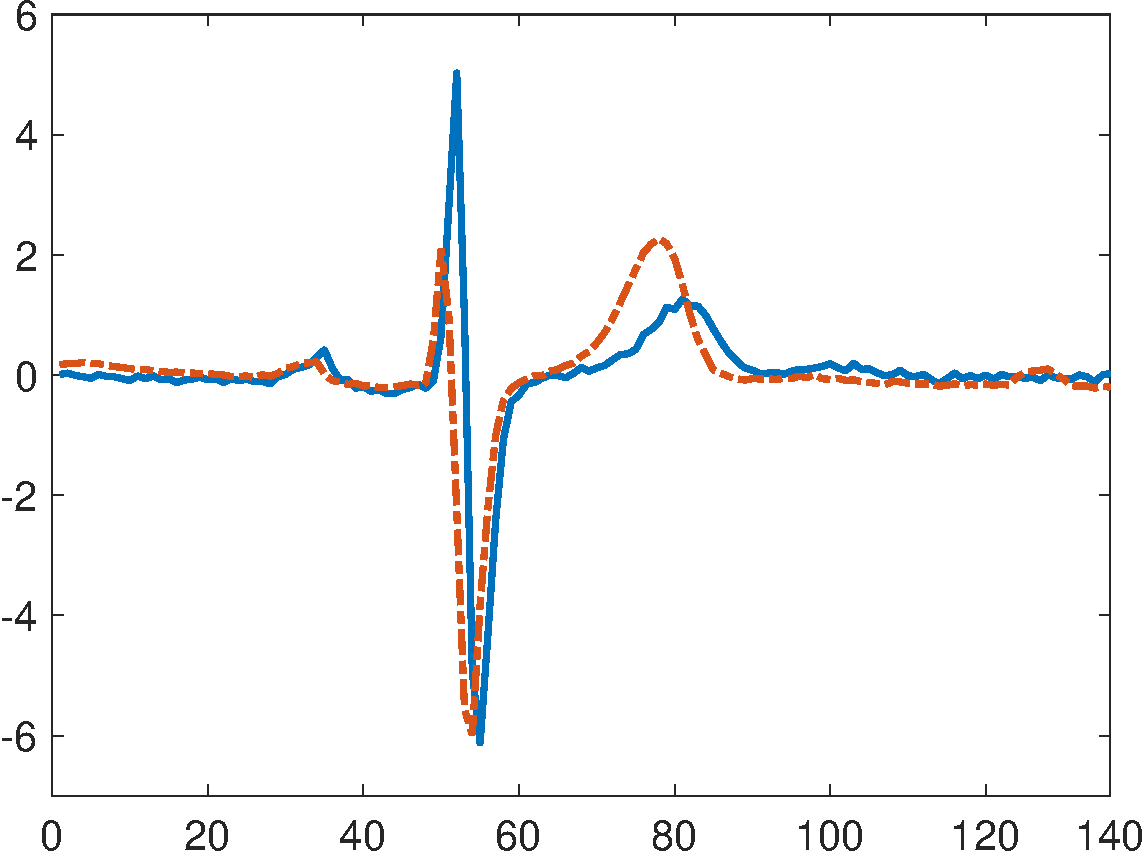
\includegraphics[height=2cm,width=4.3cm]{figures/Normzscore-crop.pdf}
	}}%
	%\qquad
	\subfloat[MinMax]{{\label{fig:norm2}}{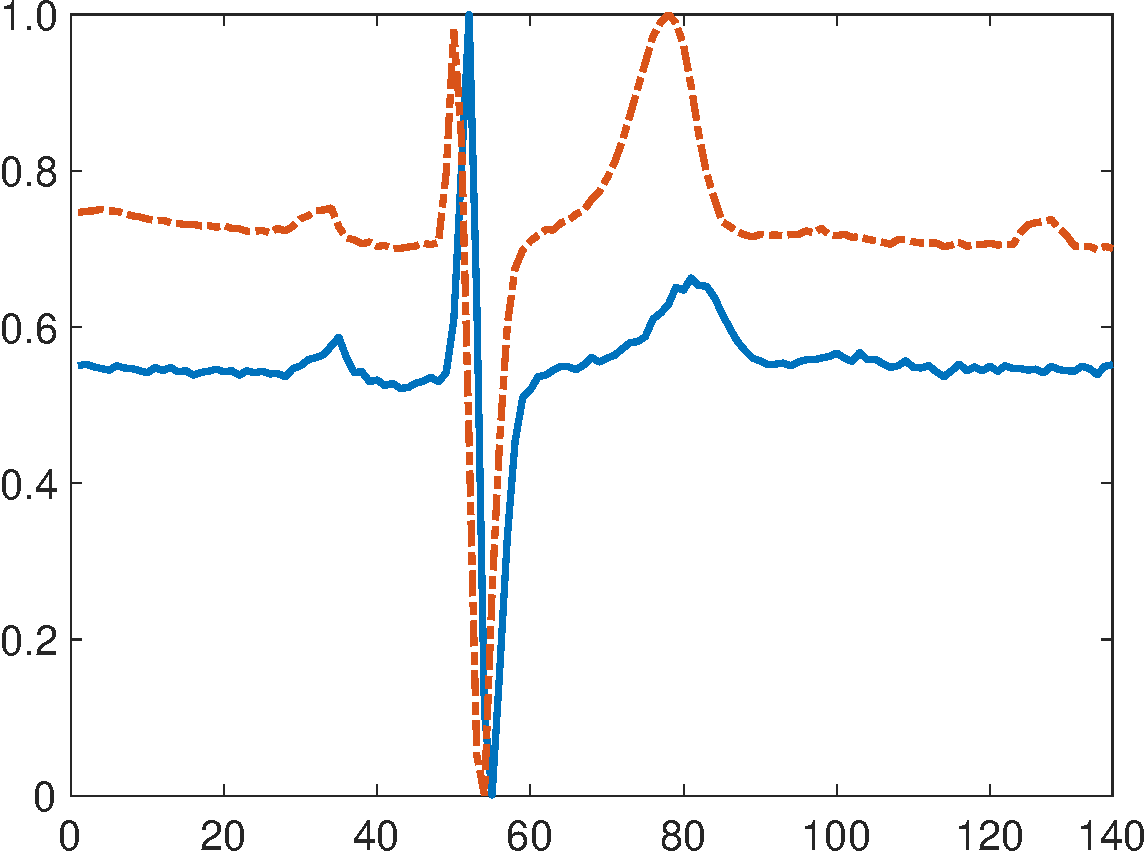
\includegraphics[height=2cm,width=4.3cm]{figures/Normminmax-crop.pdf}
	}} 
		\subfloat[UnitLength]{{\label{fig:norm3}}{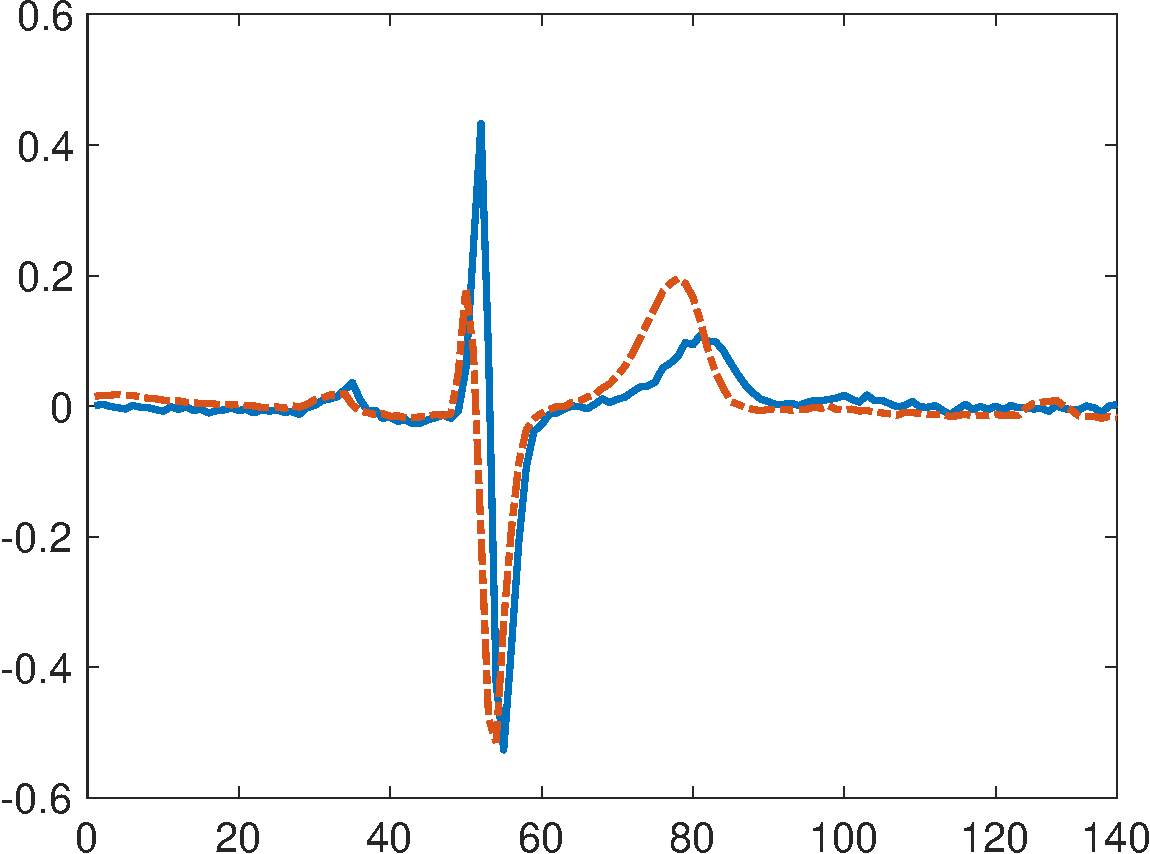
\includegraphics[height=2cm,width=4.3cm]{figures/Normunitlength-crop.pdf}
	}} 
		\subfloat[MeanNorm]{{\label{fig:norm4}}{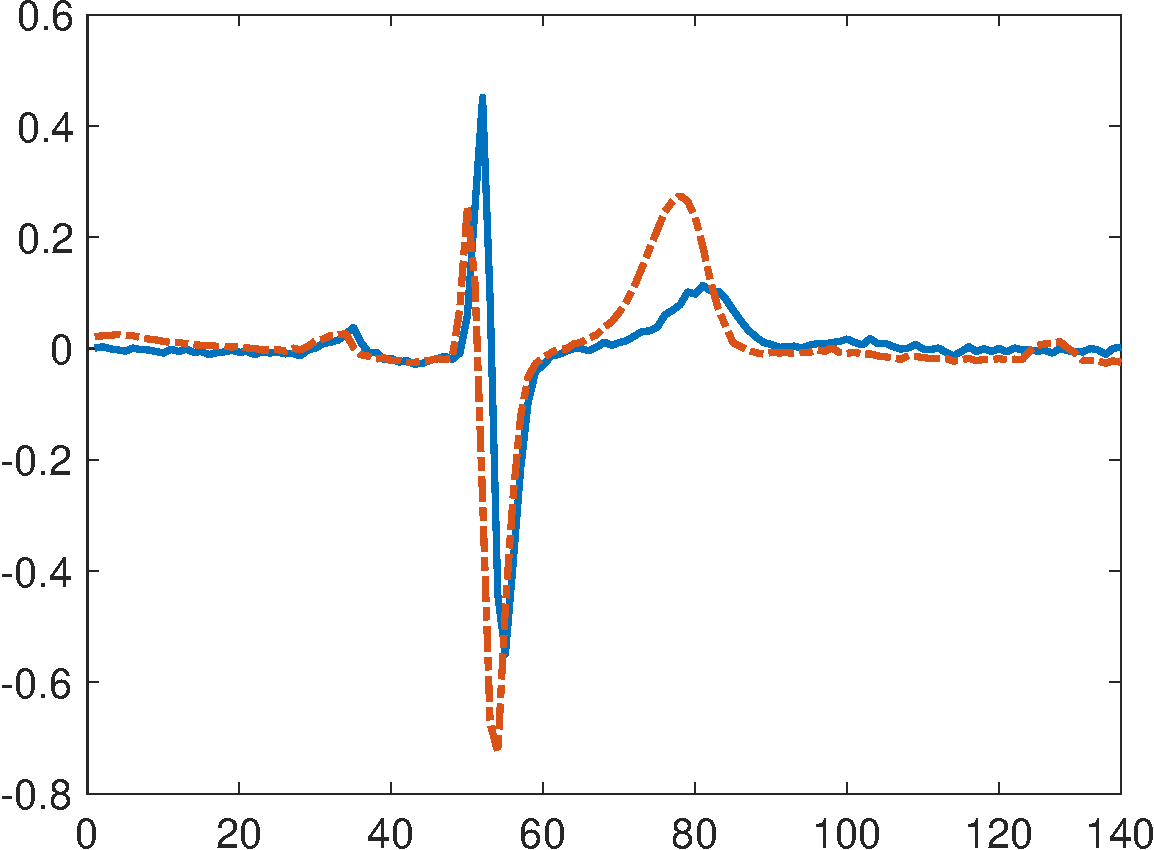
\includegraphics[height=2cm,width=4.3cm]{figures/Normmeannorm-crop.pdf}
	}} \vspace*{-0.3cm}
	\qquad
		\subfloat[MedianNorm]{{\label{fig:norm5}}{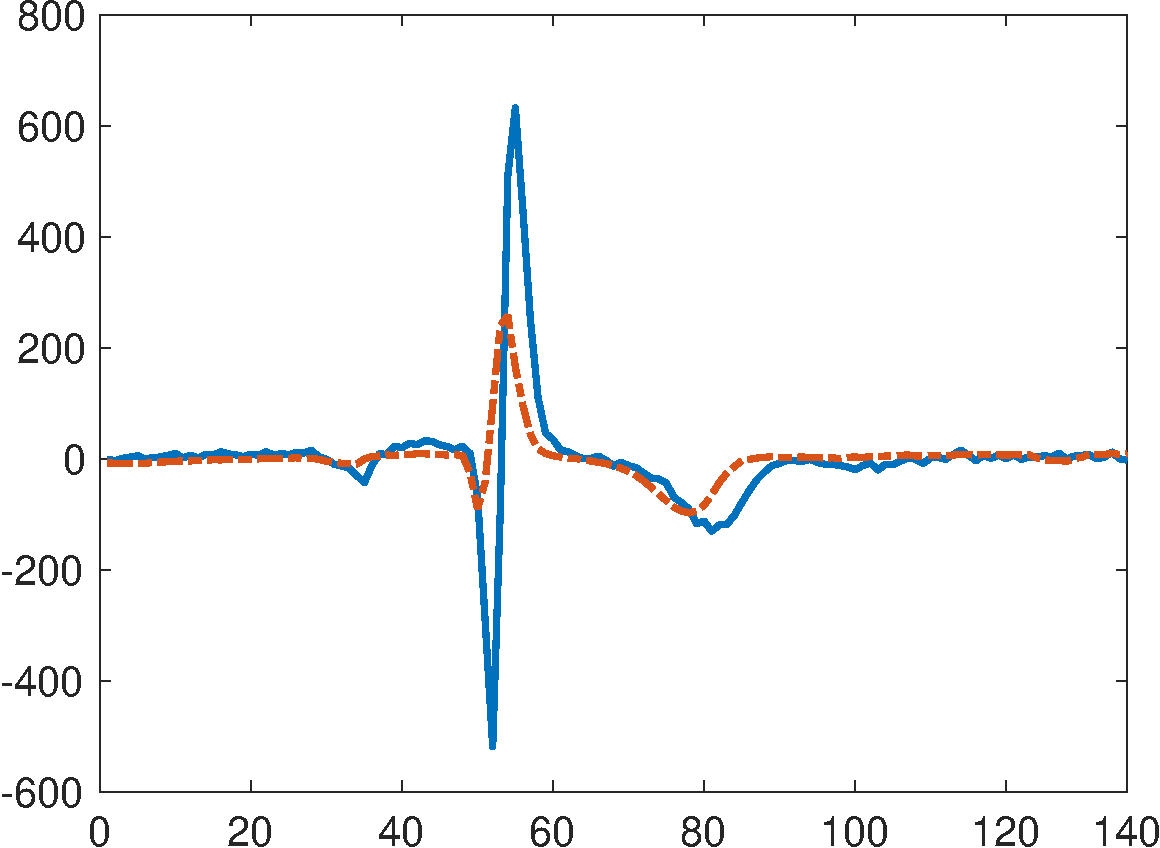
\includegraphics[height=2cm,width=4.3cm]{figures/Normmediannorm-crop.pdf}
	}} 
		\subfloat[AdaptiveScaling]{{\label{fig:norm6}}{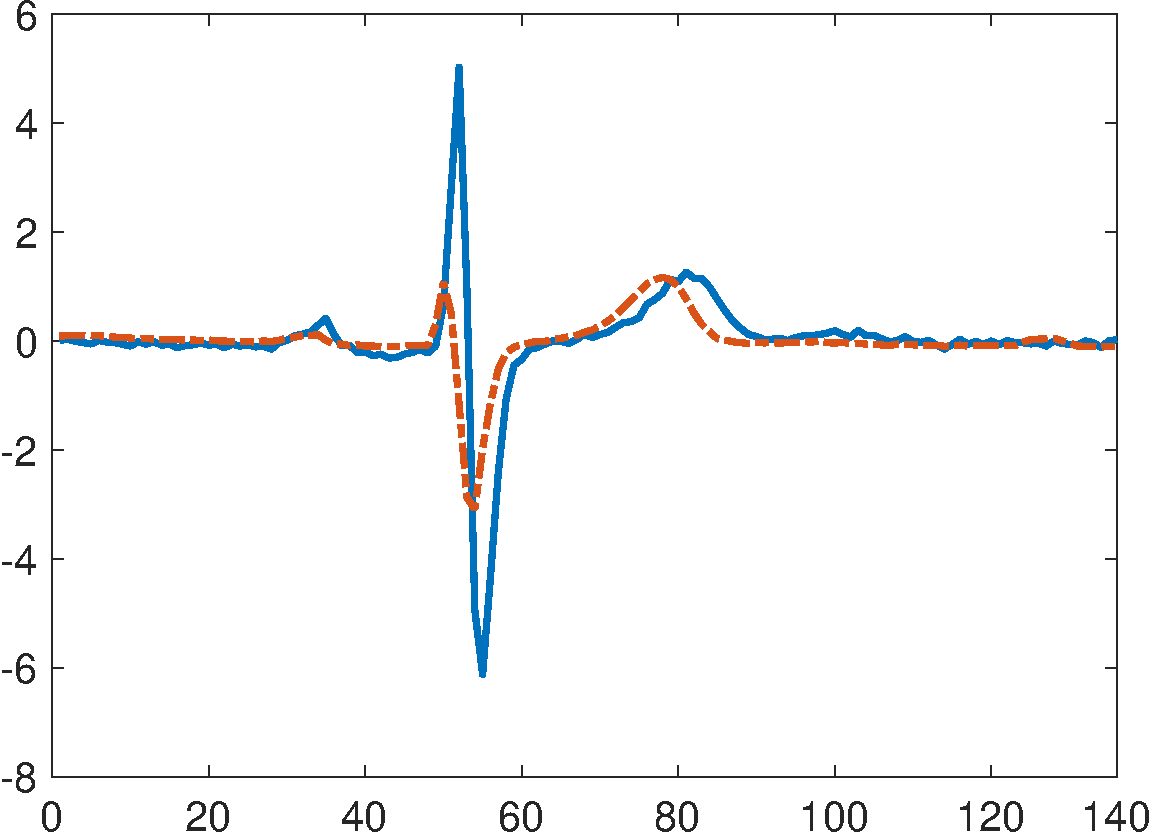
\includegraphics[height=2cm,width=4.3cm]{figures/Normadaptive-crop.pdf}
	}} 
		\subfloat[Logistic]{{\label{fig:norm7}}{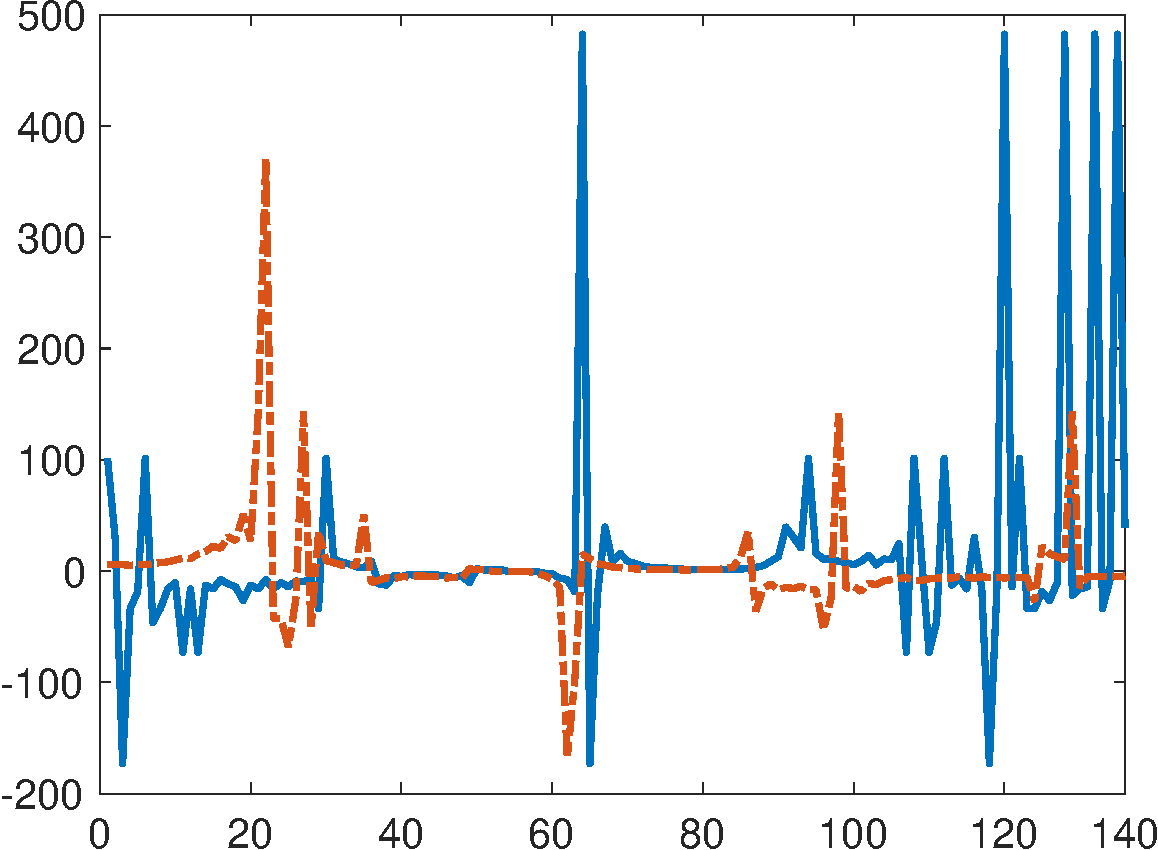
\includegraphics[height=2cm,width=4.3cm]{figures/Normsigmoid-crop.pdf}
	}} 
		\subfloat[Tanh]{{\label{fig:norm8}}{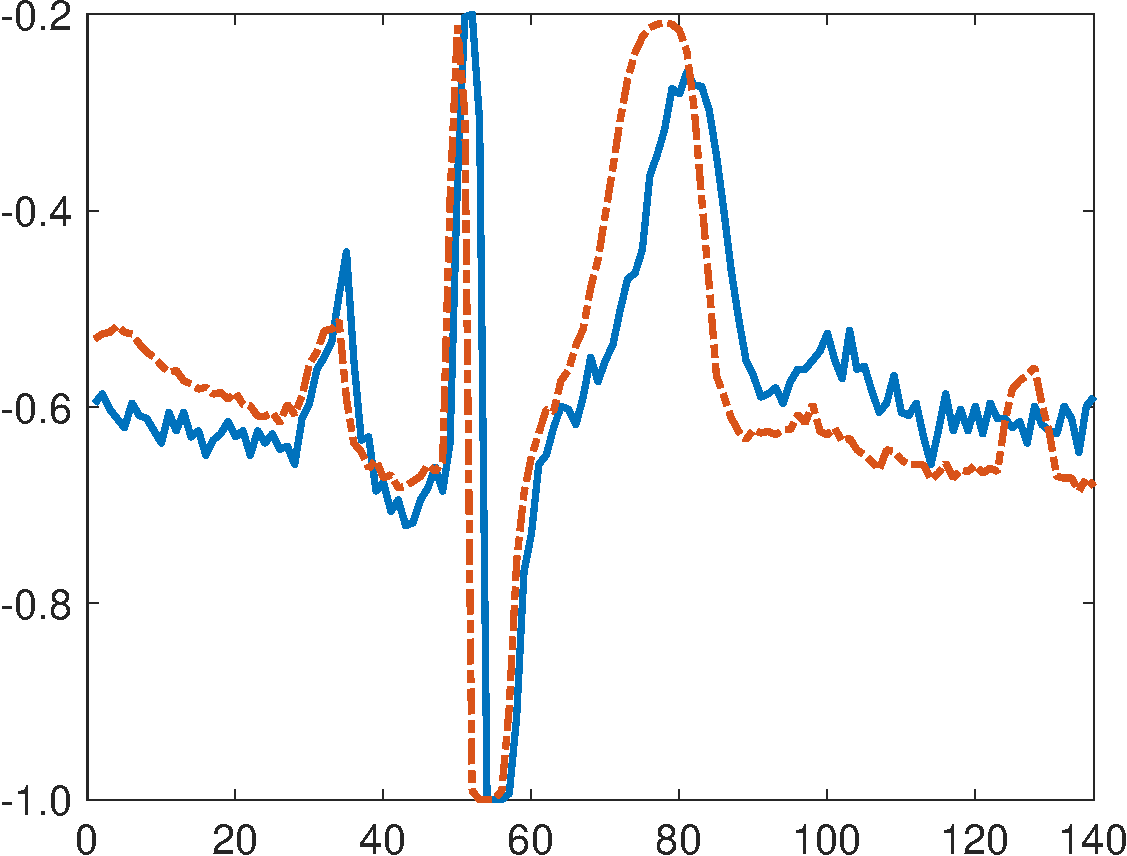
\includegraphics[height=2cm,width=4.3cm]{figures/Normtanh-crop.pdf}
	}} 
	\vspace*{-0.2cm}
	\caption{Example of how each of the $8$ normalization methods transforms two time series of the ECGFiveDays dataset \cite{UCRArchive2018}.}%
    %\vspace*{-0.2cm}
	\label{fig:normalizations}%
\end{figure*}

%\vspace*{-0.1cm}
\section{Time-Series Normalizations}
\label{sec:normalizations}
In this section, we review $8$ normalization methods usually performed as a preprocessing step before any comparison.

As we discussed earlier, a critical issue when comparing time series is how to handle a number of distortions that are characteristic of the time series. For complex distortions, sophisticated distance measures are required as offering invariances to such distortions is not trivial, which explains the proliferation of distance measures in the literature. However, in several cases, a simple preprocessing step is generally sufficient to eliminate particular distortions, as we see next.

Consider the following two examples \cite{goldin1995similarity}: (i) two products with similar sales patterns but different sales volume; and (ii) temperatures of two days starting at different values but exhibiting the exact same pattern. The first is an example of the difference in {\em scale} between two time series, whereas the second is an example of the difference in {\em translation}. Despite such differences, in many cases, it is useful to recognize the similarity between time series. Formally, for any constants $a$ (scale) and $b$ (translation), linear transformations in time series of the form $a\vec{x}+b$ should not affect their similarity. 

Several methods have been proposed to handle these popular distortions. {\em Normalization} methods transform the data to become normally distributed, whereas {\em standardization} methods place different data ranges on a common scale. In the machine-learning literature, feature {\em scaling} is also used to refer to such methods. In practice, all terms are used interchangeably to refer to some data transformation.
\newline \textbf{$Z$-score normalization: } The most popular normalization method in the time-series literature is by far the $z$-score (see Section \ref{sec:perceptions}). $Z$-score transforms data such that the resulting distribution has zero-mean and unit-variance:
\vspace{-0.12cm}
\begin{equation}
\label{eq:zscore}
\centering
\vec{x}'=\frac{\vec{x}-average(\vec{x})}{std(\vec{x})}
\vspace{-0.12cm}
\end{equation}
where $average(\cdot)$ is the mean of $\vec{x}$ and $std(\cdot)$ is its standard deviation. $Z$-score is also widely used in many machine-learning algorithms, which might explain its popularity \cite{grus2019data}.
\newline \textbf{Min-max normalization (MinMax): } An alternative approach is to scale time-series values in the [0,1] range: 
\vspace{-0.1cm}
\begin{equation}
\label{eq:minmax}
\centering
\vec{x}'=\frac{\vec{x}-min(\vec{x})}{max(\vec{x})-min(\vec{x})}
\vspace{-0.1cm}
\end{equation}
However, many distance measures cannot deal with zero values and, therefore, scaling time series between an arbitrary set of values [a,b] is often preferred:
\vspace{-0.1cm}
\begin{equation}
\label{eq:minmax2}
\centering
\vec{x}'=a+\frac{\vec{x}-min(\vec{x})\cdot(b-a)}{max(\vec{x})-min(\vec{x})}
\vspace{-0.1cm}
\end{equation}
The selection of the range is data-dependent and might require tuning to maximize its effectiveness.
\newline \textbf{Mean normalization (MeanNorm): } Another option to normalize time series is to combine the previous methods: 
\vspace{-0.1cm}
\begin{equation}
\label{eq:meannorm}
\centering
\vec{x}'=\frac{\vec{x}-average(\vec{x})}{max(\vec{x})-min(\vec{x})}
\vspace{-0.1cm}
\end{equation}
such that numerator is based on $z$-score and the denominator is based on MinMax normalization.
\newline \textbf{Median normalization (MedianNorm): } Another method is to divide the data points by the median (or mean): 
\vspace{-0.1cm}
\begin{equation}
\label{eq:mediannorm}
\centering
\vec{x}'=\frac{\vec{x}}{median(\vec{x})}
\vspace{-0.1cm}
\end{equation}
which is less popular due to numerical issues that may arise.
\newline \textbf{Unit length normalization (UnitLength): } A common way to normalize time series is to scale the data points such that the whole time series has length one:
\vspace{-0.1cm}
\begin{equation}
\label{eq:unitlength}
\centering
\vec{x}'=\frac{\vec{x}}{||\vec{x}||}
\vspace{-0.1cm}
\end{equation}
where $||\cdot||$ denotes the Euclidean norm.
\newline \textbf{Adaptive scaling (AdaptiveScaling)) \cite{chu1999fast,yang2011patterns}: } In contrast to all previous normalization methods, this approach computes the scaling factor between pairs of time series: 
\vspace{-0.1cm}
\begin{equation}
\label{eq:adaptivescaling}
\centering
a = \frac{\vec{x_i}\cdot\vec{x_j}^{T}}{\vec{x_i}\cdot\vec{x_j}^{T}}
\vspace{-0.1cm}
\end{equation}
which is used in each pairwise comparison (e.g., ED($\vec{x_i}$,$a\cdot\vec{x_j}$).

Recently, several activation functions for neural networks gained popularity \cite{lecun2012efficient}. We explore two such functions.
\newline \textbf{Logistic or sigmoid normalization (Logistic)): } The logistic function uses the formula below to activate time series: 
\vspace{-0.1cm}
\begin{equation}
\label{eq:logistic}
\centering
\vec{x}' = \frac{1}{1+e^{-\vec{x}}}
\vspace{-0.1cm}
\end{equation}
\textbf{Hyperbolic tangent normalization (Tanh)): } This method uses the formula below to activate time-series values: 
\vspace{-0.1cm}
\begin{equation}
\label{eq:logistic}
\centering
\vec{x}' = \frac{e^{2\vec{x}}-1}{e^{2\vec{x}}+1}
\vspace{-0.1cm}
\end{equation}

Figure \ref{fig:normalizations}, shows an example of how each one of the previously described normalization methods transforms a pair of time series from the ECGFiveDays dataset \cite{UCRArchive2018}. We observe that in some cases, the differences are only visible in the range of values (e.g., $z$-score vs. UnitLength), but, in others, the visual effect is more distinct (e.g., MinMax, MeanNorm, and AdaptiveScaling). The most unexpected visual effects come from the two non-linear transformations (i.e., Logistic and Tanh). We evaluate the accuracy of these $8$ methods along with the $52$ lock-step measures in the next section.

\section{Time-Series Lock-Step Distances}
\label{sec:lockstep}

In this section, we study $52$ lock-step measures that have been proposed across different scientific disciplines.

Distance measures provide a numerical value to quantify how distant are pairs of objects represented as points, vectors, or matrixes. Due to the difficulty in formalizing the notion of similarity, as well as the need to handle a variety of distortions and applications, hundreds of distance measures have been proposed in the literature. This proliferation of distance measures across different scientific areas has resulted in multi-year efforts to organize this knowledge into dictionaries \cite{deza2006dictionary} and encyclopedias \cite{deza2009encyclopedia} of distance measures. 

As it is understandable, not all of these measures are applicable to time-series data. Thankfully, different endeavors have already been conducted to identify appropriate measures for a variety of tasks across different fields \cite{zezula2006similarity,gavin2003statistical}. An influential study \cite{cha2007comprehensive} identified $50$ lock-step distance measures that we adapt in our evaluation of time-series distance measures. We note that a previous study \cite{giusti2013empirical} evaluated a subset of these measures ($45$) using $1$-NN over $42$ datasets from the UCR archive and concluded that there is no significant differences between these lock-step distance measures.

Unfortunately, we identified issues with this study. First, several of the evaluated measures are known to be equivalent to each other and, therefore, they should provide identical classification accuracy results. For example, this is the case for the Euclidean distance and the inner product (or Pearson's correlation), which under $z$-normalization, they should provide the same accuracy numbers. Second, several distance measures were not properly implemented, resulting in using as distance values either the real part of complex numbers or the first value of a normalized vector of the input time series. Therefore, the analysis of these lock-step measures is incomplete, and the findings of the study are inconclusive.

In our study, we have carefully re-implemented all $50$ distance measures from \cite{cha2007comprehensive}. The distance measures belong to $7$ different families of measures: (1) $4$ measures belong to the $L_p$ Minkowski family; (2) $6$ measures belong to the $L_1$ family; (3) $7$ measures belong to the {\em Intersection} family; (4) $6$ measures belong to the {\em Inner Product} family; (5) $5$ measures belong to the {\em Fidelity} family; (6) $8$ measures belong to the $L_2$ family; and (7) $6$ measures belong to the {\em Entropy} family. Apart from these $42$ measures, we also consider the $3$ measures that utilize ideas from multiple other measures ({\em Combinations}) as well as $5$ measures proposed in the survey but not reported in the literature (until that point), overall $50$ measures.
\begin{table}[]
\small
\centering
\begin{tabular}{|c|c|c|c|c|c|c|}
\hline
\textbf{\begin{tabular}[c]{@{}c@{}}Distance \\ Measure\end{tabular}} & \textbf{\begin{tabular}[c]{@{}c@{}}Scaling \\ Method\end{tabular}} & \textbf{\begin{tabular}[c]{@{}c@{}}Better\end{tabular}} & \textbf{\begin{tabular}[c]{@{}c@{}}Average \\ Accuracy\end{tabular}} & \textbf{\textgreater{}} & \textbf{=} & \textbf{\textless{}} \\ \hline
\multirow{5}{*}{\begin{tabular}[c]{@{}c@{}}Minkowski \\ ($L_{p}$-norm)\end{tabular}} 
&$z$-score& \textcolor{ForestGreen}{\ding{52}}&	0.7083& 79& 13& 36 \\ \cline{2-7} 
&MinMax& \textcolor{ForestGreen}{\ding{52}}& 0.7041& 70& 12& 46 \\ \cline{2-7} 
&UnitLength& \textcolor{ForestGreen}{\ding{52}}& 0.7083& 79& 13& 36 \\ \cline{2-7} 
&MeanNorm& \textcolor{ForestGreen}{\ding{52}}& 0.7082& 81& 10& 37 \\ \cline{2-7} 
&Tanh& \textcolor{BrickRed}{\ding{56}}& 0.6941& 60& 7& 61 \\ \hline





\multirow{5}{*}{Lorentzian} 
&$z$-score& \textcolor{ForestGreen}{\ding{52}}& 0.7022& 71& 8& 49 \\ \cline{2-7}
&MinMax& \textcolor{ForestGreen}{\ding{52}}& 0.7010& 66& 7& 55 \\ \cline{2-7}
&UnitLength& \textcolor{ForestGreen}{\ding{52}}& 0.7024& 76& 9& 43 \\ \cline{2-7}
&MeanNorm& \textcolor{ForestGreen}{\ding{52}}& 0.7061& 75& 9& 44 \\ \cline{2-7}
&Tanh& \textcolor{BrickRed}{\ding{56}}& 0.6950& 63& 9&56 \\ \hline



	
	
\multirow{6}{*}{\begin{tabular}[c]{@{}c@{}}Manhattan \\ ($L_{1}$-norm)\end{tabular}} 
&$z$-score&	\textcolor{ForestGreen}{\ding{52}}&	0.7017&	76&	11&	41 \\ \cline{2-7} 
&MinMax&	\textcolor{ForestGreen}{\ding{52}}&	0.7017&	66&	11&	51 \\ \cline{2-7} 
&UnitLength&	\textcolor{ForestGreen}{\ding{52}}&	0.7017&	76&	11&	41 \\ \cline{2-7} 
&MeanNorm&	\textcolor{ForestGreen}{\ding{52}}&	0.7051&	76&	9&43 \\ \cline{2-7} 
&Tanh&	\textcolor{BrickRed}{\ding{56}}&	0.6913&	63&	11&	54 \\ \hline





\multirow{5}{*}{Avg $L_{1}$/$L_{\infty}$} 
&$z$-score&	\textcolor{ForestGreen}{\ding{52}}&	0.7012&	75&	10&	43 \\ \cline{2-7} 
&MinMax&	\textcolor{ForestGreen}{\ding{52}}&	0.7013&	68&	5&	55 \\ \cline{2-7} 
&UnitLength&	\textcolor{ForestGreen}{\ding{52}}&	0.7012&	75&	10&	43 \\ \cline{2-7} 
&MeanNorm&	\textcolor{ForestGreen}{\ding{52}}&	0.7046&	76&	9&	43 \\ \cline{2-7} 
&Tanh&	\textcolor{BrickRed}{\ding{56}}&	0.6911&	60&	13&	55 \\ \hline



\multirow{5}{*}{DISSIM} 
&$z$-score&	\textcolor{ForestGreen}{\ding{52}}&	0.7013&	78&	6&	44 \\ \cline{2-7} 
&MinMax&	\textcolor{ForestGreen}{\ding{52}}&	0.7016&	66&	8&	54 \\ \cline{2-7} 
&UnitLength&	\textcolor{ForestGreen}{\ding{52}}&	0.7013&	78&	6&	44 \\ \cline{2-7} 
&MeanNorm& \textcolor{ForestGreen}{\ding{52}}&	0.7039&	73&	9&	46 \\ \cline{2-7} 
&Tanh&	\textcolor{BrickRed}{\ding{56}}&	0.6917&	64&	10&	54 \\ \hline



\multirow{2}{*}{Jaccard} 
&MinMax&	\textcolor{BrickRed}{\ding{56}}&	0.6955&	66&	12&	50 \\ \cline{2-7}
&MeanNorm&	\textcolor{ForestGreen}{\ding{52}}&	0.6939&	76&	19&	33 \\ \hline




\multirow{2}{*}{\begin{tabular}[c]{@{}c@{}}ED \\ ($L_{2}$-norm)\end{tabular}} 
&MinMax&	\textcolor{BrickRed}{\ding{56}}&	0.6947&	69&	13&	46 \\ \cline{2-7} 
&MeanNorm&	\textcolor{BrickRed}{\ding{56}}&	0.6896&	67&	11&	50 \\ \hline


Emanon4 & MinMax&	\textcolor{ForestGreen}{\ding{52}}&	0.7034&	72&	6&	50  \\ \hline
Soergel & MinMax&	\textcolor{ForestGreen}{\ding{52}}&	0.7011&	73&	4&	51  \\ \hline
Clark & MinMax&	\textcolor{BrickRed}{\ding{56}}&	0.6986&	73&	4&	51  \\ \hline
Topsoe & MinMax&	\textcolor{BrickRed}{\ding{56}}&	0.6962&	71&	4&	53  \\ \hline
Chord & MinMax&	\textcolor{BrickRed}{\ding{56}}&	0.6934&	64&	8&	56 \\ \hline
ASD & MinMax& \textcolor{BrickRed}{\ding{56}}&	0.6884&	56&	13&	59 \\ \hline
Canberra & MinMax&	\textcolor{BrickRed}{\ding{56}}&	0.6933&	56&	4&	68  \\ \hline

\hline
\textbf{ED} & \textbf{$z$-score} & \textbf{-} & \textbf{0.6863} & \textbf{-} &	\textbf{-} & \textbf{-} \\ \hline
\end{tabular}
\caption{\textcolor{black}{Comparison of lock-step distance measures. ``Scaling Method'' column indicates the underlying time-series normalization. ``Better'' column denotes that the distance measure outperforms the baseline with statistical significance. ``Average Accuracy'' column shows the mean accuracy achieved across $128$ datasets. The last three columns indicate the number of datasets over which a distance measure is better (``>''), equal (``=''), or worse (``<'') than the baseline.}
}
\label{table:lockstep}
\vspace{-0.2cm}
\end{table}

Besides these measures, we also include two measures that have substantial differences from the previous lock-step measures. Specifically, DISSIM \cite{frentzos2007index} defines the distance as a definite integral of the function of time of the ED in order to take into consideration different sampling rates of time series. This computationally expensive operation can be approximated by a modified version of ED that considers in the distance of the $i$th points the $i+1$th points, which is a form of a smoothing operation. Finally, the adaptive scaling distance (ASD), embeds internally the AdaptiveScaling normalization described previously with an inner product measure to compare time series under optimal scaling \cite{chu1999fast,yang2011patterns}. \textcolor{black}{We exclude from our analysis and leave for future study three recently proposed correlation-aware measures \cite{mirylenka2017data} that are more complex in nature than those we consider here.}
\newline \textbf{Evaluation of lock-step measures: } In lieu of including several pages with formulas and tables with raw classification accuracy numbers, we created a website to ease the exploration of our results, as noted earlier. For all mathematical formulas, we refer the reader to the previous survey \cite{cha2007comprehensive}. Below, we only report the summary of raw results and findings from our rigorous statistical analysis. Specifically, we evaluate $52$ distance measures and their combinations with $8$ normalization methods using our $1$-NN classifier over $128$ datasets (see Section \ref{sec:preliminaries}). Table \ref{table:parameters} contains all distance measures requiring parameter tuning along with the evaluated parameters. From the lock-step measures,
only one measure, the Minkowski distance, requires tuning.

Table \ref{table:lockstep} reports the performance of lock-step measures against the baseline listed in the last row. Following the convention \cite{fernandez2014we}, we also report the average accuracy across datasets but we note that this number is meaningless when not accompanied by rigorous statistical analysis. Specifically, from all combinations of distance measures and normalization methods ($52\cdot8=416$ in total), we only report those resulting in an average accuracy higher than the one achieved by ED with $z$-score, the current state-of-the-art lock-step measure. We omit measures achieving the same or worse average accuracy than ED. We observe $14$ measures with some improvement in their average accuracy in contrast to ED and overall $36$ combinations with different normalization methods. However, only about half of these combinations result in statistically significant differences according to the Wilcoxon test. (We perform all pairwise comparisons with Wilcoxon to ensure we did not miss any accurate measure.) 

\begin{figure} \centering 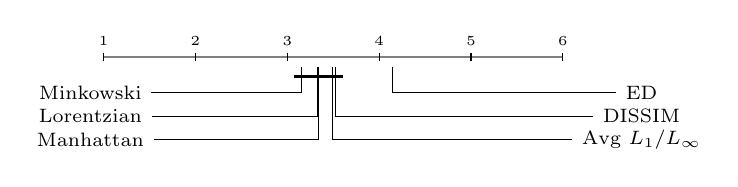
\begin{tikzpicture}[xscale=2]
\draw[gray, thick](00.5833, 0) -- (03.5000, 0);
\foreach \x in {00.5833,01.1667,01.7500,02.3333,02.9167,03.5000}\draw (\x cm,1.5pt) -- (\x cm, -1.5pt);
\node (Label) at (00.5833,0.2) {\tiny{1}};
\node (Label) at (01.1667,0.2) {\tiny{2}};
\node (Label) at (01.7500,0.2) {\tiny{3}};
\node (Label) at (02.3333,0.2) {\tiny{4}};
\node (Label) at (02.9167,0.2) {\tiny{5}};
\node (Label) at (03.5000,0.2) {\tiny{6}};
\draw[decorate,decoration={amplitude=.4mm,segment length=1.5mm,post length=0mm}, very thick, color = black](01.7910,-00.2500) -- ( 02.1051,-00.2500);
\node (Point) at (01.8410, 0){};  \node (Label) at (0.5,-00.4500){\scriptsize{Minkowski}}; \draw (Point) |- (Label);
\node (Point) at (01.9437, 0){};  \node (Label) at (0.5,-00.7500){\scriptsize{Lorentzian}}; \draw (Point) |- (Label);
\node (Point) at (01.9507, 0){};  \node (Label) at (0.5,-01.0500){\scriptsize{Manhattan}}; \draw (Point) |- (Label);
\node (Point) at (02.4197, 0){};  \node (Label) at (4.0,-00.4500){\scriptsize{ED}}; \draw (Point) |- (Label);
\node (Point) at (02.0551, 0){};  \node (Label) at (4.0,-00.7500){\scriptsize{DISSIM}}; \draw (Point) |- (Label);
\node (Point) at (02.0393, 0){};  \node (Label) at (4.0,-01.0500){\scriptsize{Avg $L_{1}$/$L_{\infty}$}}; \draw (Point) |- (Label);
\end{tikzpicture}
\vspace{-0.3cm}
\caption{\textcolor{black}{Ranking of lock-step measures under $z$-score based on the average of their ranks across datasets.}}
\label{fig:zscoremanymeasures}
\vspace{-0.5cm}
\end{figure}

\begin{figure} \centering 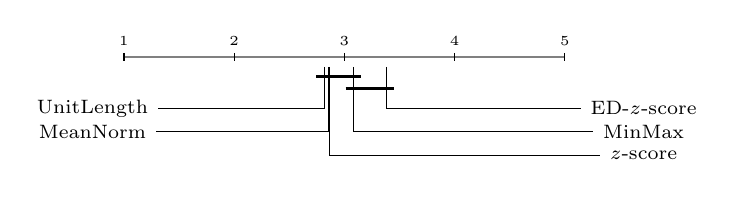
\begin{tikzpicture}[xscale=2]
\draw[gray, thick](00.7000, 0) -- (03.5000, 0);
\foreach \x in {00.7000,01.4000,02.1000,02.8000,03.5000}\draw (\x cm,1.5pt) -- (\x cm, -1.5pt);
\node (Label) at (00.7000,0.2) {\tiny{1}};
\node (Label) at (01.4000,0.2) {\tiny{2}};
\node (Label) at (02.1000,0.2) {\tiny{3}};
\node (Label) at (02.8000,0.2) {\tiny{4}};
\node (Label) at (03.5000,0.2) {\tiny{5}};
\draw[decorate,decoration={amplitude=.4mm,segment length=1.5mm,post length=0mm}, very thick, color = black](01.9212,-00.2500) -- ( 02.2074,-00.2500);
\draw[decorate,decoration={amplitude=.4mm,segment length=1.5mm,post length=0mm}, very thick, color = black](02.1074,-00.4000) -- ( 02.4153,-00.4000);
\node (Point) at (01.9712, 0){};  \node (Label) at (0.5,-00.6500){\scriptsize{UnitLength}}; \draw (Point) |- (Label);
\node (Point) at (02.0013, 0){};  \node (Label) at (0.5,-00.9500){\scriptsize{MeanNorm}}; \draw (Point) |- (Label);
\node (Point) at (02.3653, 0){};  \node (Label) at (4.0,-00.6500){\scriptsize{ED-$z$-score}}; \draw (Point) |- (Label);
\node (Point) at (02.1574, 0){};  \node (Label) at (4.0,-00.9500){\scriptsize{MinMax}}; \draw (Point) |- (Label);
\node (Point) at (02.0041, 0){};  \node (Label) at (4.0,-01.2500){\scriptsize{$z$-score}}; \draw (Point) |- (Label);
\end{tikzpicture}
\vspace{-0.3cm}
\caption{\textcolor{black}{Ranking of normalization methods in combination with the Lorentzian distance based on the average of their ranks across datasets. ED uses $z$-score normalization.}}
\label{fig:lorentziandifferentnorms}
\vspace{-0.2cm}
\end{figure}

In particular, Minkowski distance performs better in terms of average accuracy than all other distance measures, but it is also the only measure that requires tuning, which is not always desirable. Interestingly, several measures of the $L_{1}$ family, namely, the Lorentzian (i.e., the natural logarithm of $L_{1}$), the Manhattan, and the Avg $L_{1}$/$L_{\infty}$, outperform ED with statistically significant differences. DISSIM, a measure that integrates some form of smoothing of time series, also outperforms ED significantly. In all of these measures, we observe a similar trend: all combinations with $z$-score, UnitLength, and MeanNorm normalizations lead to significant improvements. However, our extensive experimentation reveals \textcolor{black}{three unknown measures in the time-series literature that achieve statistically significant improvement over ED, namely, the Jaccard distance with MeanNorm, the Emanon4 distance with MinMax, and the Soergel distance with MinMax}. Interestingly, all three distance measures do not show improvements under $z$-score, which shows the importance of considering different normalizations. Among all methods, MeanNorm seems to perform the best. However, the Wilcoxon test suggests no statistically significant differences between any of the $17$ combinations that outperform ED with $z$-score.




To better understand the performance of lock-step measures, we also evaluate the significance of their differences in accuracy when considering several distance measures together, using the Friedman test followed by a post-hoc Nemenyi test. Specifically, we perform two analyses: (i) we evaluate different distance measures under the same normalization; and (ii) we evaluate standalone distance measures under different normalizations; Figure \ref{fig:zscoremanymeasures} shows the average rank across all datasets of the distance measures, which under $z$-score normalization, outperformed previously ED. The thick line connects measures that do not perform statistically significantly better. We observe that Lorentzian is ranked first (once we ignore the supervised Minkowski), meaning that it performed best in the majority of the datasets. All $5$ measures significantly outperform ED, but we observe no difference between them. Figure \ref{fig:lorentziandifferentnorms} evaluates a standalone distance measure, the Lorentzian measure that performed the best previously, with different normalization methods against ED with $z$-score. We observe that the $3$ out of the $4$ combinations that were better than ED under the Wilcoxon test remain better under this statistical analysis, and there is no difference between them. We omit similar figures for the other measures as we observe the similar trends.

\noindent \textbf{Debunking $\mathcal{M}1$ and $\mathcal{M}2$: } Our evaluation shows clear evidence that normalization methods other than $z$-score can lead to significant improvements, which debunks $\mathcal{M}1$. Even though for standalone measures, we did not observe significant improvements (e.g.,  ED with MeanNorm vs. ED with $z$-score), that does not reject our hypothesis. We note that the majority of the UCR datasets are in their $z$-normalized form and, therefore, for fairness, we $z$-normalized all datasets, which may have limited this analysis. Despite that, we identified two new distance measures, unknown until now, that only under MinMax and MeanNorm methods outperform ED with $z$-score and, importantly, $z$-score is not suitable for them. Normalizations such as MeanNorm, which combines $z$-score and MinMax methods, seems to perform the best for several measures. Similarly, our analysis shows that distance measures other than ED can lead to significant improvements, which debunks $\mathcal{M}2$. We identified $7$ distance measures that significantly outperform ED. We emphasize that no previous study considered different normalization methods in order to challenge $\mathcal{M}1$, and our findings contradict both previous studies \cite{ding2008querying,giusti2013empirical}, which concluded that there is no significant difference in the accuracy of lock-step measures.

Next, we focus on sliding versions of lock-step measures. 
\vspace*{-0.1cm}
\section{Time-Series Sliding Distances}
\label{sec:sliding}

We study $4$ variants of cross-correlation, a measure that has largely been omitted from distance measure evaluations. 

Starting with the concurrent introduction of lock-step and elastic measures for the problem of time-series similarity search \cite{agrawal1993,Faloutsos1994fast,berndt1994using}, the vast majority of research focused on these two categories of measures (see $\mathcal{M}3$ in Section \ref{sec:perceptions}). Cross-correlation, which is similar to convolution, dates back in the 1700s \cite{dominguez2015history} but received practical popularity only after the invention of Fast Fourier Transform (FFT) \cite{cooley1965algorithm}, which dramatically reduced its computational cost. Cross-correlation is one of the most fundamental operations in signal processing \cite{brown1992survey} and, lately, in deep neural networks \cite{lecun1995convolutional,lecun2015deep}. Recently, research focusing on time-series clustering used cross-correlation and achieved state-of-the-art performance for this task \cite{paparrizos2015k,paparrizos2017fast}. However, this work assumed $z$-normalized time series and performed evaluations only against ED and DTW. Next, we present cross-correlation following the notation used in \cite{paparrizos2015k} in an attempt to establish consistent terminology with the recent literature.

In simple terms, the cross-correlation measure maximizes the correlation \textcolor{black}{(or, equivalently, minimizes the ED \cite{FastestSimilaritySearch})} between a time-series $\vec{x}$ and all shifted versions of another time series $\vec{y}$. By shifting (or sliding), we refer to an operation, $\vec{x}_{(s)}$, that rearranges the data points by moving all points by $|s|$ positions to the right, for $s\geq0$, or left, for $s<0$. For example, $\vec{x}_{(1)}$ moves all data points by one position to the right and brings the final entry to the first position (or differently pads the empty positions with zeros; both approaches lead to similar measures). When we consider all shifts, $s \in [-m,m]$, where $m$ is the length of both time series (the measure can also operate with unequal lengths), we produce the cross-correlation sequence, $CC_{w}(\vec{x},\vec{y})$, with $w \in \{1,2,\ldots, 2m-1\}$, of length $(2m-1)$, containing the inner product of the two time series in every possible shift. 

\begin{table}[]
\setlength{\tabcolsep}{4.3pt}
\small
\centering
\begin{tabular}{|c|c|c|c|c|c|c|}
\hline
\textbf{\begin{tabular}[c]{@{}c@{}}Distance \\ Measure\end{tabular}} & \textbf{\begin{tabular}[c]{@{}c@{}}Scaling \\ Method\end{tabular}} & \textbf{\begin{tabular}[c]{@{}c@{}}Better\end{tabular}} & \textbf{\begin{tabular}[c]{@{}c@{}}Average \\ Accuracy\end{tabular}} & \textbf{\textgreater{}} & \textbf{=} & \textbf{\textless{}} \\ \hline
\multirow{7}{*}{\begin{tabular}[c]{@{}c@{}}NCC$_c$ \\ (SBD)\end{tabular}} 
&$z$-score& \textcolor{ForestGreen}{\ding{52}}&	0.7309& 86&9&33 \\ \cline{2-7} 

&MinMax& \textcolor{ForestGreen}{\ding{52}}& 0.7186&72&8&48\\ \cline{2-7} 

&UnitLength& \textcolor{ForestGreen}{\ding{52}}& 0.7309&86&9&33 \\ \cline{2-7} 

&MeanNorm& \textcolor{ForestGreen}{\ding{52}}& 0.7309&86&9&33 \\ \cline{2-7} 

&MedianNorm& \textcolor{BrickRed}{\ding{56}}& 0.7050&63&7&58 \\ \cline{2-7} 

&Adaptive& \textcolor{BrickRed}{\ding{56}}& 0.7072&72&8&48 \\ \cline{2-7} 

&Tanh& \textcolor{BrickRed}{\ding{56}}& 0.7077&58&8&62 \\ \hline


\multirow{2}{*}{NCC$_b$} &$z$-score& \textcolor{ForestGreen}{\ding{52}}& 0.7309&86&9&33 \\ \cline{2-7}

&UnitLength& \textcolor{ForestGreen}{\ding{52}}&0.7309&86&9&33\\ \hline



\multirow{2}{*}{NCC} &$z$-score&	\textcolor{ForestGreen}{\ding{52}}&	0.7309&86&9&33 \\ \cline{2-7} 
&UnitLength&	\textcolor{ForestGreen}{\ding{52}}&	0.7309&86&9&33 \\ \hline




\hline
\textbf{Lorentzian} & \textbf{UnitLength} & \textbf{-} & \textbf{0.7024} & \textbf{-} &	\textbf{-} & \textbf{-} \\ \hline
\end{tabular}
\caption{\textcolor{black}{Comparison of sliding distance measures. ``Scaling Method'' column indicates the underlying time-series normalization. ``Better'' column denotes that the distance measure outperforms the baseline with statistical significance. ``Average Accuracy'' column shows the mean accuracy achieved across $128$ datasets. The last three columns indicate the number of datasets over which a distance measure is better (``>''), equal (``=''), or worse (``<'') than the baseline.}
}
\label{table:sliding}
\vspace{-0.1cm}
\end{table}

Unfortunately, the computation of $CC_{w}(\vec{x},\vec{y})$ is expensive, $\mathcal{O}(m^2)$, but, thankfully, with the use of FFT ($\mathcal{F}(\cdot)$) and its inverse version ($\mathcal{F}^{-1}(\cdot))$, the cost reduces to $\mathcal{O}(m\cdot\log(m))$:
%\vspace{-0.1cm}
\begin{equation}
\label{eq:ifftfft}
\centering
CC_{w}(\vec{x},\vec{y})  =
\mathcal{F}^{-1}\{\mathcal{F}(\vec{x}) * \mathcal{F}(\vec{y})\}
%\vspace{-0.1cm}
\end{equation}
Having introduced the necessary notation and considering popular normalizations, we can derive the following 4 variants of cross-correlation similarity measures \cite{paparrizos2015k}:
%\vspace{-0.15cm}
\begin{equation}
\label{eq:ncc}
  NCC_{q}(\vec{x},\vec{y})=\begin{cases}
    \max\left(\frac{CC_{w}(\vec{x},\vec{y})}{m}\right), &\text{$q=``b"$ ($NCC_{b}$)}\\
    %\\
    \max\left( \frac{CC_{w}(\vec{x},\vec{y})}{m-|w-m|}\right), &\text{$q=``u"$ ($NCC_{u}$)}\\
    %\\
    \max\left(\frac{CC_{w}(\vec{x},\vec{y})}{||\vec{x}||\cdot||\vec{y}||}\right), &\text{$q=``c"$ ($NCC_{c}$)}\\
    \max(CC_{w}(\vec{x},\vec{y})), &\text{$q=``\cdot"$ ($NCC$)}
  \end{cases}
  %\vspace{-0.15cm}
\end{equation}
known as the normalized cross-correlation (because it assumes some underlying time-series normalization), $NCC$, the biased estimator, $NCC_{b}$, the unbiased estimator, $NCC_{u}$, and the coefficient normalization or SBD \cite{paparrizos2015k}, $NCC_{c}$.
\newline \textbf{Evaluation of sliding measures: } Due to the resemblance of cross-correlation to the sliding version of Pearson's correlation, when time series are $z$-normalized, the majority of the literature assumes this underlying data normalization \cite{paparrizos2015k}. To the best of our knowledge, the performance of cross-correlation as a measure to compare time series under different normalization methods is not well explored. Table \ref{table:sliding} reports the performance of the combinations of cross-correlation variants with normalization methods. Specifically, from 32 such combinations (i.e., $4$ measures $\times$ $8$ normalizations), we report only those resulted in an average accuracy higher than the one achieved by Lorentzian (with $z$-score followed by UnitLength, the last row of the Table \ref{table:sliding}), the new state-of-the-art lock-step distance measure based on our previous analysis (Section \ref{sec:lockstep}). As before, we perform all pairwise comparisons using the Wilcoxon statistical test to ensure we did not miss any accurate combination.

We observe that from all $4$ cross-correlation measures, the unbiased estimator, $NCC_{u}$, performs worse than all other variants. Specifically, no combination of $NCC_{u}$ with any of the normalization methods outperforms the Lorentzian distance. In contrast, the remaining $3$ variants, $NCC$, $NCC_{b}$, and $NCC_{c}$, all include combinations that outperform the baseline. In particular, combinations of $NCC$ and $NCC_{b}$ with $z$-score and UnitLength normalizations significantly outperform the baseline. We observe negligible differences between these combinations (i.e., only one dataset is slightly affected). Interestingly, the coefficient normalization variant, $NCC_{c}$, outperforms the baseline with $6$ combinations of normalization methods. However, only half of these combinations outperform the Lorentzian distance with a statistically significant difference. In all of these measures, we observe a similar trend: all combinations with $z$-score and UnitLength normalization methods lead to significant improvements. However, for $NCC_{c}$, another normalization, namely, MeanNorm, also achieves similar improvement, which is not the case when combined with $NCC$ and $NCC_{b}$. Even though $NCC$, $NCC_{b}$, and $NCC_{c}$ perform similarly in terms of average accuracy, $NCC_{c}$ appears to be the most robust cross-correlation measure as it leads to improvement over the baseline with more normalization methods than the other variants and for three such combinations the improvement is statistically significant. Among all combinations that outperform the baseline, Wilcoxon suggests no statistically significant differences.

\begin{figure} \centering 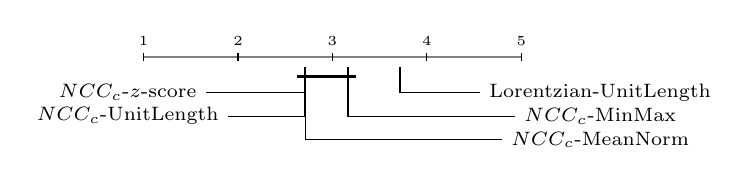
\begin{tikzpicture}[xscale=2]
\draw[gray, thick](00.6000, 0) -- (03.0000, 0);
\foreach \x in {00.6000,01.2000,01.8000,02.4000,03.0000}\draw (\x cm,1.5pt) -- (\x cm, -1.5pt);
\node (Label) at (00.6000,0.2) {\tiny{1}};
\node (Label) at (01.2000,0.2) {\tiny{2}};
\node (Label) at (01.8000,0.2) {\tiny{3}};
\node (Label) at (02.4000,0.2) {\tiny{4}};
\node (Label) at (03.0000,0.2) {\tiny{5}};
\draw[decorate,decoration={amplitude=.4mm,segment length=1.5mm,post length=0mm}, very thick, color = black](01.5718,-00.2500) -- ( 01.9484,-00.2500);
\node (Point) at (01.6218, 0){};  \node (Label) at (0.5,-00.4500){\scriptsize{$NCC_{c}$-$z$-score}}; \draw (Point) |- (Label);
\node (Point) at (01.6218, 0){};  \node (Label) at (0.5,-00.7500){\scriptsize{$NCC_{c}$-UnitLength}}; \draw (Point) |- (Label);
\node (Point) at (02.2290, 0){};  \node (Label) at (3.5,-00.4500){\scriptsize{Lorentzian-UnitLength}}; \draw (Point) |- (Label);
\node (Point) at (01.8984, 0){};  \node (Label) at (3.5,-00.7500){\scriptsize{$NCC_{c}$-MinMax}}; \draw (Point) |- (Label);
\node (Point) at (01.6290, 0){};  \node (Label) at (3.5,-01.0500){\scriptsize{$NCC_{c}$-MeanNorm}}; \draw (Point) |- (Label);
\end{tikzpicture}
\vspace{-0.3cm}
\caption{\textcolor{black}{Ranking of different normalization methods for $NCC_{c}$ based on the average of their ranks across datasets, using Lorentzian with UnitLength as the baseline method.}}
\label{fig:sliding1}
\vspace{-0.2cm}
\end{figure}







In addition to these pairwise comparisons, we also evaluate the significance of the differences when considered all together. Figure \ref{fig:sliding1} shows the average rank across datasets of five combinations of $NCC_{c}$ with normalization methods (we excluded Tanh normalization as from Table \ref{table:sliding} we observe that, despite the increase in average accuracy, the Lorentzian distance still outperforms this combination in more datasets). Similarly to the pairwise analysis, we observe that combinations with $z$-score, MeanNorm, and UnitLength normalizations lead to significant improvements according to the Friedman test followed by a post-hoc Nemenyi test to assess the significance of the differences in the ranking. Combinations of $NCC_{c}$ with AdaptiveScaling or MinMax do not achieve significant improvement. We observe that both statistical evaluation approaches lead to similar conclusions. We omit figures for $NCC$ and $NCC_{b}$ with similar findings.

For completeness, we report another analysis using ED as the baseline instead of the Lorentzian distance (we omit the figure due to space limitation). $NCC_{c}$ in combination with $z$-score, UnitLength, and MeanNorm normalization methods outperform ED but, in contrast to Figure \ref{fig:sliding1}, now combinations with AdaptiveScaling and MinMax are also significantly better than ED. This analysis confirms our results in Section \ref{sec:lockstep} that the Lorentzian distance (and other $L_{1}$ variants) are more powerful than ED. In addition, our analysis indicates that $NCC_{c}$ outperforms all lock-step measures with all different normalizations, making it a strong baseline method for time-series comparison.

\begin{table}[]
\setlength{\tabcolsep}{4.3pt}
\small
\centering
\begin{tabular}{cl}
\hline
\textbf{\begin{tabular}[c]{@{}c@{}}Distance \\ Measure\end{tabular}}     & \textbf{Parameters} \\
\hline
MSM       & $c \in \{0.01,0.1,1,10,100,0.05,0.5,5,50,500\}$         \\ \hline
DTW       & \begin{tabular}[c]{@{}l@{}}$\delta \in \{0,1,2,3,4,5,6,7,8,9,10,11,12,13,14,15,16,$ \\
                  $17,18,19,20,100\}$\end{tabular}           \\ \hline
EDR       & \begin{tabular}[c]{@{}l@{}}$\epsilon \in \{0.001,0.003,0.005,0.007,0.009,0.01,0.03,0.05,$ \\
$0.07,0.09,0.1,0.2,0.3,0.4,0.5,0.6,0.7,0.8,0.9,1\}$ \end{tabular}           \\ \hline
LCSS & \begin{tabular}[c]{@{}l@{}}$\delta \in \{5,10\}$ \\
$\epsilon\in \{0.001,0.003,0.005,0.007,0.009,0.01,0.03,0.05,$ \\
$0.07,0.09,0.1,0.2,0.3,0.4,0.5,0.6,0.7,0.8,0.9,1\}$ \end{tabular}            \\ \hline
TWE & \begin{tabular}[c]{@{}l@{}}$\lambda \in \{0,0.25,0.5,0.75,1.0\}$ \\
$\nu \in \{0.00001,0.0001,0.001,0.01,0.1,1\}$ \end{tabular}            \\ \hline
Swale & \begin{tabular}[c]{@{}l@{}}$\epsilon \in \{0.01,0.03,0.05,0.07,0.09,0.1,0.2,0.3,0.4,0.5,$ \\
$0.6,0.7,0.8,0.9,1\}, p \in \{5\}, r \in \{1\}$\end{tabular}            \\ \hline
Minkowski & \begin{tabular}[c]{@{}l@{}}$p \in \{0.1,0.3,0.5,0.7,0.9,1,1.3,1.5,1.7,1.9,$ \\
$2,3,5,7,9,11,13,15,17,20\}$ \end{tabular}            \\ \hline

\textcolor{black}{KDTW} & \begin{tabular}[c]{@{}l@{}}$\gamma \in \{2^{-15},2^{-14},2^{-13},2^{-12},2^{-11},2^{-10},2^{-9},2^{-8},$ \\ $2^{-7},2^{-6},2^{-5},2^{-4},2^{-3},2^{-2},2^{-1},2^0\}$ \end{tabular}            \\ \hline

\textcolor{black}{GAK} & \begin{tabular}[c]{@{}l@{}}$\gamma \in \{0.01,0.05,0.1,0.25,0.5,0.75,1,2,3,4,$ \\
$5,6,7,8,9,10,11,12,13,14,15,16,17,18,19,20\}$ \end{tabular}            \\ \hline

\textcolor{black}{SINK} & \begin{tabular}[c]{@{}l@{}}$\gamma \in \{1,2,3,4,5,6,7,8,9,10,11,12,13,14,15,16,$ \\
$17,18,19,20\}$ \end{tabular}            \\ \hline

\textcolor{black}{RBF} & \begin{tabular}[c]{@{}l@{}}$\gamma \in \{2^{-15},2^{-14},2^{-13},2^{-12},2^{-11},2^{-10},2^{-9},2^{-8},2^{-7},$ \\ $2^{-6},2^{-5},2^{-4},2^{-3},2^{-2},2^{-1},2^0\}$ \end{tabular}   \\ \hline

\textcolor{black}{GRAIL} & \begin{tabular}[c]{@{}l@{}}$\gamma \in \{1,2,3,4,5,6,7,8,9,10,11,12,13,14,15,16,$ \\
$17,18,19,20\}$ \end{tabular}   \\ \hline

\textcolor{black}{RWS} & \begin{tabular}[c]{@{}l@{}}$\gamma \in \{10^{-3}, 3\cdot10^{-3}, 10^{-2}, 3\cdot10^{-2}, 0.1, 0.14, 0.19,$ \\ 
$0.28, 0.39, 0.56, 0.79, 1.12, 1.58, 2.23, 3.16, 4.46, 6.30,$ \\
$8.91, 10, 31.62, 10^2, 3\cdot10^2, 10^3\}$, $D_{max}=25$ \end{tabular}   \\ \hline

\textcolor{black}{SIDL} & \begin{tabular}[c]{@{}l@{}}$\lambda \in \{0.1, 1, 10\}$, $r \in \{0.1, 0.25, 0.5\}$  \end{tabular}   \\ 

\hline
\end{tabular}
\caption{\textcolor{black}{Parameter choices for distance measures.}.}
\label{table:parameters}
\vspace{-0.4cm}
\end{table}

We now turn our focus to elastic measures and, particularly, to their performance against sliding measures.

\section{Time-Series Elastic Measures}
\label{sec:elastic}

In this section, we study $7$ elastic measures, a popular category of measures for time-series comparison.

As discussed earlier, sliding measures find a global alignment by sliding one time series against the other. In contrast, elastic measures create a non-linear mapping between time-series data points to support flexible alignment of different regions. Through this mapping, elastic measures permit time series to ``stretch'' or ``shrink'' their observations to improve time-series matching. Most elastic measures rely on dynamic programming to find this mapping efficiently by defining recursive formulas over a $m$-by-$m$ matrix $M$ that contains in each cell the ED (or some other lock-step measure) between every point of one time series against every point of another time series. In general, the goal of different elastic measures in the literature is to employ different strategies to find a {\em warping path}, $W=\{w_1,\ldots,w_k\}$, with $k\geq m$, a contiguous set of matrix cells that shows the mapping of every point of one time series to one, more, or none of the points of the other time series. To improve the efficiency and the accuracy of elastic measures, it is a common practice to introduce constraints (in the form of parameters) to guide the warping path to visit only a subset of cells in $M$ or to determine above which distance threshold two points should match.

The first elastic measure, DTW \cite{sakoe1971dynamic,sakoe1978dynamic}, was proposed as a speech recognition tool and, later, it was introduced in the time-series literature as a suitable approach for time-series comparison \cite{berndt1994using}. DTW finds the warping path that minimizes the distances between all data points. In the original form, DTW is parameter-free, however, many approaches have been proposed to define {\em bands} (i.e., the shape of the subset cells of matrix $M$ that the warping path is permitted to visit) and the {\em width or window} (i.e., size) of the bands. We use the Sakoe-Chiba band \cite{sakoe1978dynamic}, which is the most frequently used in practice \cite{ding2008querying}, and we tune the window $\delta$ using parameters shown in Table \ref{table:parameters}. For example, a value $\delta=10$ indicates a window size $10\%$ of the time-series length. 

\begin{table}[]
\setlength{\tabcolsep}{4.5pt}
\small
\centering
\begin{tabular}{|c|c|c|c|c|c|c|}
\hline
\textbf{\begin{tabular}[c]{@{}c@{}}Distance \\ Measure\end{tabular}} & \textbf{\begin{tabular}[c]{@{}c@{}}Parameter \\ Tuning\end{tabular}} & \textbf{\begin{tabular}[c]{@{}c@{}}Better\end{tabular}} & \textbf{\begin{tabular}[c]{@{}c@{}}Average \\ Accuracy\end{tabular}} & \textbf{\textgreater{}} & \textbf{=} & \textbf{\textless{}} \\ \hline
\multirow{2}{*}{\begin{tabular}[c]{@{}c@{}}MSM\end{tabular}} 

&LOOCCV& \textcolor{ForestGreen}{\ding{52}}&	0.7628&86&3&39 \\ \cline{2-7} 

& $c=0.5$& \textcolor{ForestGreen}{\ding{52}}& 0.7627&89&2&37\\ \hline

\multirow{2}{*}{TWE} &LOOCCV& \textcolor{ForestGreen}{\ding{52}}& 0.7632&85&4&39 \\ \cline{2-7}

&$\lambda\!=\!1,\!\nu\!=\!0.0001$& \textcolor{ForestGreen}{\ding{52}}& 0.7622&89&4&35 \\ \hline

\multirow{3}{*}{DTW} &LOOC& \textcolor{ForestGreen}{\ding{52}}& 0.7519&75&16&37 \\ \cline{2-7}

&$\delta=100$& \textcolor{BrickRed}{\ding{56}}&0.7248&54&10&64 \\ \cline{2-7} 
&$\delta=10$& \textcolor{BrickRed}{\ding{56}}& 0.7372&64&6&58 \\ \hline

\multirow{2}{*}{EDR} &LOOCCV& \textcolor{ForestGreen}{\ding{52}}& 0.7485&74&8&46 \\ \cline{2-7}

&$\epsilon=0.1$ & \textcolor{BrickRed}{\ding{56}}& 0.7202&62&5&61 \\ \hline


\multirow{2}{*}{Swale} &LOOCCV& \textcolor{ForestGreen}{\ding{52}}& 0.7499&72&8&48 \\ \cline{2-7}

&$\epsilon=0.2$ & \textcolor{BrickRed}{\ding{56}}& 0.7229&63&4&61 \\ \hline

ERP & - & \textcolor{ForestGreen}{\ding{52}}& 0.7488&77&5&46 \\ \hline


\multirow{2}{*}{LCSS} &LOOCCV& \textcolor{BrickRed}{\ding{56}}& 0.7398&66&6&56 \\ \cline{2-7}

&$\delta=5,\epsilon=0.2$& \textcolor{BrickRed}{\ding{56}}& 0.7160&63&2&63 \\ \hline
\hline
\textbf{NCC$_{c}$} & \textbf{-} & \textbf{-} & \textbf{0.7309} & \textbf{-} &	\textbf{-} & \textbf{-} \\ \hline
\end{tabular}
\caption{\textcolor{black}{Comparison of elastic measures against $NCC_c$. ``Parameter Tuning'' indicates supervised or unsupervised tuning. ``Better'' denotes that the measure outperforms the baseline with statistical significance. ``Average Accuracy'' shows the mean accuracy achieved across $128$ datasets. The last three columns indicate the datasets over which a measure is better (``>''), equal (``=''), or worse (``<'') than the baseline.}
}
\label{table:elastic1}
\vspace{-0.4cm}
\end{table}

The Longest Common Subsequence (LCSS) distance is another type of elastic measure that was derived from the idea of edit-distances for characters. Specifically, LCSS introduces a parameter $\epsilon$ that serves as a threshold to determine when two points of time series should match \cite{andre1997using,vlachos2002discovering}. Similarly to DTW, LCSS also constrains the warping window by introducing an additional parameter $\delta$ \cite{vlachos2002discovering}. Edit Distance on Real sequence (EDR) distance \cite{chen2005robust} is another edit-distance-based measure that similarly to LCSS, uses a parameter $\epsilon$ to quantify the distance of points as $0$ or $1$. EDR also introduces penalties for gaps between matched subsequences. Edit Distance with Real Penalty (ERP) distance \cite{chen2004marriage} is a measure that bridges DTW and EDR distance measures by more carefully computing the distance between gaps of time series.

Differently than the previous approaches, the Sequence Weighted Alignment model (Swale) \cite{morse2007efficient} proposes a model to compute the similarity of time series using rewards for matching points and penalties for gaps. Apart from a threshold $\epsilon$ parameter, Swale also requires parameters for the reward $r$ and the penalty $p$. The Move–split–merge (MSM) distance \cite{stefan2013move} is another elastic measure based on edit-distance but in contrast to DTW, LCSS, and EDR, MSM is a metric. MSM uses a set of operations to replace, insert, or delete values in time series to improve their matching. Finally, Time Warp Edit (TWE) distance \cite{marteau2008time} is a measure that combines merits from LCSS and DTW. TWE introduces a stiffness parameter $\nu$ to control the warping but at the same point it also penalizes matched points (parameter $\lambda$).

For each one of these $7$ elastic measures, several variants and extensions have been proposed in the literature. For example, Derivative DTW (DDTW) \cite{gorecki2013using} combines raw time series with their first-order differences (derivatives). Complexity Invariant distance (CID) \cite{batista2014cid} is a weighting scheme to compensate for differences in the complexity of two time series. Finally, Weighted DTW (WDTW) \cite{jeong2011weighted} adds a penalty to the warping path of DTW. All of these approaches describe extensions that can potentially be used in combination with all previously described elastic measures. Importantly, each of these extensions often introduces additional parameters that require tuning. To avoid an explosion of evaluated approaches, we do not include such variants in our analysis. An excellent recent study \cite{bagnall2017great} focusing on time-series classification has evaluated several of these approaches (and did not identify significant improvements from their use). 
\newline \textbf{Evaluation of elastic vs. sliding measures: } With the introduction of the $7$ elastic measures we are now in position to evaluate their performance against sliding measures, an experiment that has been omitted in all previous studies \cite{ding2008querying,bagnall2017great}. Table \ref{table:elastic1} compares the classification accuracy of elastic measures against the accuracy of $NCC_{c}$, the state-of-the-art sliding measure based on our previous experiment in Section \ref{sec:sliding}. As we did not observe significant differences from using different normalization methods for $NCC_{c}$, for all subsequent experiments we always use $z$-normalized time series. We also do that so that our results are closely comparable to those reported previously \cite{ding2008querying,wang2013experimental}. Table \ref{table:elastic1} includes two experimental settings, one supervised and one unsupervised. In the supervised setting, the necessary parameters of the elastic measures are tuned on the training set using cross-validation with a leave-one-out-classifier (LOOCCV), as noted in Section \ref{sec:preliminaries}. In the unsupervised setting, we consult the parameters selected through LOOCCV to identify a set of parameters that perform well on average across all datasets. This step involves several trial-and-error attempts and a post-hoc analysis of the results (i.e., we observe the accuracy on the test sets). Even though this is an unfair advantage against parameter-free approaches, such as $NCC_c$, we perform this post-hoc analysis to ensure that elastic measures are not misrepresented in such unsupervised scenario and that a domain expert could potentially identify such parameters without supervised tuning. For some measures, such as DTW, that was an easy step, however, for others, we had to perform multiple attempts to identify parameters that achieve a competitive accuracy on average.

\begin{figure} \centering 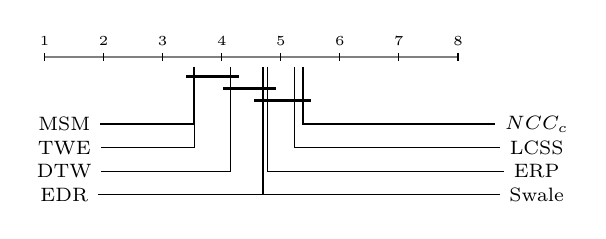
\begin{tikzpicture}[xscale=2]
\draw[gray, thick](00.3750, 0) -- (03.0000, 0);
\foreach \x in {00.3750,00.7500,01.1250,01.5000,01.8750,02.2500,02.6250,03.0000}\draw (\x cm,1.5pt) -- (\x cm, -1.5pt);
\node (Label) at (00.3750,0.2) {\tiny{1}};
\node (Label) at (00.7500,0.2) {\tiny{2}};
\node (Label) at (01.1250,0.2) {\tiny{3}};
\node (Label) at (01.5000,0.2) {\tiny{4}};
\node (Label) at (01.8750,0.2) {\tiny{5}};
\node (Label) at (02.2500,0.2) {\tiny{6}};
\node (Label) at (02.6250,0.2) {\tiny{7}};
\node (Label) at (03.0000,0.2) {\tiny{8}};
\draw[decorate,decoration={amplitude=.4mm,segment length=1.5mm,post length=0mm}, very thick, color = black](01.2726,-00.2500) -- ( 01.6070,-00.2500);
\draw[decorate,decoration={amplitude=.4mm,segment length=1.5mm,post length=0mm}, very thick, color = black](01.5070,-00.4000) -- ( 01.8414,-00.4000);
\draw[decorate,decoration={amplitude=.4mm,segment length=1.5mm,post length=0mm}, very thick, color = black](01.7065,-00.5500) -- ( 02.0656,-00.5500);
\node (Point) at (01.3226, 0){};  \node (Label) at (0.5,-00.8500){\scriptsize{MSM}}; \draw (Point) |- (Label);
\node (Point) at (01.3271, 0){};  \node (Label) at (0.5,-01.1500){\scriptsize{TWE}}; \draw (Point) |- (Label);
\node (Point) at (01.5570, 0){};  \node (Label) at (0.5,-01.4500){\scriptsize{DTW}}; \draw (Point) |- (Label);
\node (Point) at (01.7565, 0){};  \node (Label) at (0.5,-01.7500){\scriptsize{EDR}}; \draw (Point) |- (Label);
\node (Point) at (02.0156, 0){};  \node (Label) at (3.5,-00.8500){\scriptsize{$NCC_c$}}; \draw (Point) |- (Label);
\node (Point) at (01.9627, 0){};  \node (Label) at (3.5,-01.1500){\scriptsize{LCSS}}; \draw (Point) |- (Label);
\node (Point) at (01.7914, 0){};  \node (Label) at (3.5,-01.4500){\scriptsize{ERP}}; \draw (Point) |- (Label);
\node (Point) at (01.7666, 0){};  \node (Label) at (3.5,-01.7500){\scriptsize{Swale}}; \draw (Point) |- (Label);
\end{tikzpicture}
\vspace{-0.3cm}
\caption{\textcolor{black}{Ranking of elastic and sliding distance measures based on the average of their ranks across datasets, using supervised tuning for their parameters.}}
\label{fig:elastic1}
\vspace{-0.2cm}
\end{figure}

\begin{figure} \centering 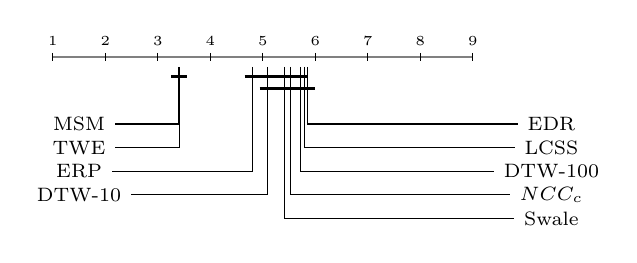
\begin{tikzpicture}[xscale=2]
\draw[gray, thick](00.3333, 0) -- (03.0000, 0);
\foreach \x in {00.3333,00.6667,01.0000,01.3333,01.6667,02.0000,02.3333,02.6667,03.0000}\draw (\x cm,1.5pt) -- (\x cm, -1.5pt);
\node (Label) at (00.3333,0.2) {\tiny{1}};
\node (Label) at (00.6667,0.2) {\tiny{2}};
\node (Label) at (01.0000,0.2) {\tiny{3}};
\node (Label) at (01.3333,0.2) {\tiny{4}};
\node (Label) at (01.6667,0.2) {\tiny{5}};
\node (Label) at (02.0000,0.2) {\tiny{6}};
\node (Label) at (02.3333,0.2) {\tiny{7}};
\node (Label) at (02.6667,0.2) {\tiny{8}};
\node (Label) at (03.0000,0.2) {\tiny{9}};
\draw[decorate,decoration={amplitude=.4mm,segment length=1.5mm,post length=0mm}, very thick, color = black](01.0840,-00.2500) -- ( 01.1853,-00.2500);
\draw[decorate,decoration={amplitude=.4mm,segment length=1.5mm,post length=0mm}, very thick, color = black](01.5517,-00.2500) -- ( 01.9563,-00.2500);
\draw[decorate,decoration={amplitude=.4mm,segment length=1.5mm,post length=0mm}, very thick, color = black](01.6467,-00.4000) -- ( 01.9980,-00.4000);
\node (Point) at (01.1340, 0){};  \node (Label) at (0.5,-00.8500){\scriptsize{MSM}}; \draw (Point) |- (Label);
\node (Point) at (01.1353, 0){};  \node (Label) at (0.5,-01.1500){\scriptsize{TWE}}; \draw (Point) |- (Label);
\node (Point) at (01.6017, 0){};  \node (Label) at (0.5,-01.4500){\scriptsize{ERP}}; \draw (Point) |- (Label);
\node (Point) at (01.6967, 0){};  \node (Label) at (0.5,-01.7500){\scriptsize{DTW-10}}; \draw (Point) |- (Label);
\node (Point) at (01.9480, 0){};  \node (Label) at (3.5,-00.8500){\scriptsize{EDR}}; \draw (Point) |- (Label);
\node (Point) at (01.9323, 0){};  \node (Label) at (3.5,-01.1500){\scriptsize{LCSS}}; \draw (Point) |- (Label);
\node (Point) at (01.9063, 0){};  \node (Label) at (3.5,-01.4500){\scriptsize{DTW-100}}; \draw (Point) |- (Label);
\node (Point) at (01.8437, 0){};  \node (Label) at (3.5,-01.7500){\scriptsize{$NCC_c$}}; \draw (Point) |- (Label);
\node (Point) at (01.8020, 0){};  \node (Label) at (3.5,-02.0500){\scriptsize{Swale}}; \draw (Point) |- (Label);
\end{tikzpicture}
\vspace{-0.3cm}
\caption{\textcolor{black}{Ranking of elastic and sliding distance measures based on the average of their ranks across datasets, using unsupervised tuning for their parameters.}}
\label{fig:elastic2}
\vspace{-0.2cm}
\end{figure}


\textcolor{black}{From Table \ref{table:elastic1}, we observe that when parameters are selected under supervised settings (lines with LOOCCV tuning) all elastic measures significantly outperform $NCC_c$ with one exception, the LCSS measure, which marginally outperforms $NCC_c$  but the difference is not statistically significant according to Wilcoxon.} However, the picture is different for the unsupervised scenario. Specifically, we observe that $4$ out of the $7$ elastic measures do not outperform $NCC_c$. Interestingly, LCSS, EDR, and DTW (with $\delta=100$, which resembles an equivalent parameter-free measure to $NCC_c$) are slightly worse. MSM, TWE, and ERP on the other side significantly outperform $NCC_c$ in the unsupervised setting as well. Among all elastic measures, ERP is the only parameter-free measure that achieves significantly better accuracy than $NCC_c$ in both supervised and unsupervised settings.

To better understand the performance of elastic measures against $NCC_c$, in addition to all previous pairwise statistical comparisons, we also evaluate the significance of the differences when considered all together. Specifically, Figure \ref{fig:elastic1} shows the average ranks of the elastic measures in the supervised setting and Figure \ref{fig:elastic2} shows the average ranks in the unsupervised setting. The ranking of measures in Figure \ref{fig:elastic1} contradicts some of the pairwise results observed in Table \ref{table:elastic1}. Specifically, we observe that even under supervised settings, $4$ out of the $7$ elastic measures, namely, LCSS, ERP, EDR, and Swale, do not achieve significantly better performance than $NCC_c$. The results for MSM, TWE, and DTW, are consistent in both statistical evaluations. For the unsupervised setting, both statistical evaluation approaches agree to an extent. In particular, Figure \ref{fig:elastic2} shows clearly that MSM and TWE outperform $NCC_c$. However, the remaining $5$ elastic measures perform similarity to $NCC_c$. Interestingly, as we observed in Table \ref{table:elastic1}, $NCC_c$ slightly outperforms $3$ elastic measures.

\textcolor{black}{To validate our findings, we repeat the analysis (we omit figures due to space limitation) and evaluate the significance of the differences when we consider all elastic measures together (i.e., excluding $NCC_c$). Specifically, we observe that Swale, ERP, EDR, and LCSS do not outperform DTW-10 with statistically significant difference. Interestingly, the supervised LCSS is slightly worse than the unsupervised DTW-10. ERP, which under pairwise evaluation appears to significantly outperform DTW-10, when all measures are considered together, both appear to achieve comparable performance. MSM, TWE, and DTW also perform similarly and all three supervised measures outperform DTW-10. However, under unsupervised settings, we observe that MSM and TWE significantly outperform all other elastic measures.}
\noindent \textbf{Debunking $\mathcal{M}3$ and $\mathcal{M}4$: } Our comprehensive evaluation shows clear evidence that sliding measures are strong baselines that most elastic measures do not manage to outperform either in supervised or unsupervised settings, which debunks $\mathcal{M}3$. Specifically, from all $5$ elastic measures evaluated in the decade-old study \cite{ding2008querying}, namely, LCSS, Swale, EDR, ERP, and DTW, only DTW significantly outperforms cross-correlation under the supervised scenario. In the unsupervised setting, none of the $5$ measures outperforms cross-correlation and, interestingly, several of them perform slightly worse. This is a remarkable finding, showing that the simplest type of alignment between time series is very effective and it should have served as a baseline method for elastic measures. Only MSM and TWE, two measures that appeared after \cite{ding2008querying} show promising results and outperform cross-correlation with statistically significant differences in both supervised and unsupervised settings. Importantly, MSM is the only method that significantly outperforms DTW under supervised settings (according to Wilcoxon) and, under unsupervised settings, both MSM and TWE significantly outperform DTW (with both statistical tests validating this result). Therefore, there is clear evidence that the widely popular DTW is no longer the best elastic distance measure, which debunks $\mathcal{M}4$. 

%\newline \textbf{Evaluation of elastic measures: } Even though the previous analysis shows some trends about the performance among elastic measures, we repeat the analysis using DTW with $\delta=10$ (DTW-10), a strong elastic measure, for baseline (we omit tables and figures due to space limitation). 

%Table \ref{table:elastic2} compares the classification accuracy of elastic measures against DTW with $\delta=10$ (DTW-10). We observe $3$ elastic measures that outperform DTW-10 when parameters are selected under supervision. Specifically, MSM, TWE, and DTW (with LOOCCV tuning) outperform DTW-10 with statistically significant difference. However, LCSS, Swale, and EDR, three supervised elastic measures, achieve comparable performance to DTW-10, an unsupervised measure. As expected, the unsupervised versions of LCSS, Swale, and EDR also do not outperform DTW-10. Interestingly, EDR appears statistically significantly worse than DTW-10 (denoted with \textcolor{NavyBlue}{\ding{74}}). This contradicts the findings of the previous study \cite{ding2008querying}, which concluded that EDR might be potentially slightly better. The unsupervised measures ERP, MSM, and TWE all appear to significantly outperform DTW-10. The DTW-100 version achieves worse performance in terms of average accuracy and, therefore, we do not include it in Table \ref{table:elastic2}. However, Wilcoxon suggests that there is no statistically significant differences between the accuracy of DTW-10 and DTW-100.

%To better understand the performance of elastic measures among each other, as before, we also evaluate the significance of the differences when considered all together. Figure \ref{fig:elastic3} shows the average ranks among elastic measures in the supervised setting whereas Figure \ref{fig:elastic3} shows the average ranks in the unsupervised setting. As before, this analysis contradicts some of the pairwise results in Table \ref{table:elastic2}. Specifically, Swale, ERP, EDR, and LCSS do not outperform DTW-10 with statistically significant difference. Interestingly, the supervised LCSS is slightly worse than the unsupervised DTW-10. ERP, which under pairwise evaluation appears to significantly outperform DTW-10, when all measures are considered together, both appear to achieve comparable performance. MSM, TWE, and DTW also perform similarly and all three supervised measures outperform DTW-10. However, the analysis under unsupervised settings show again a different picture (Figure \ref{fig:elastic4}). In particular, we observe that MSM and TWE are ranked first, significantly outperforming all other elastic measures.
\vspace{-0.2cm}
\section{Time-Series Kernel Measures}
\label{sec:kernel}
\textcolor{black}{Until now, our analysis focused on three categories of distance measures, namely, lock-step, sliding, and elastic measures, with the goal to provide answers to the four-long standing misconceptions that we discussed in Section \ref{sec:perceptions}. Recently, kernel functions \cite{scholkopf1997kernel,scholkopf1998nonlinear}, a different category of similarity measures, have started to receive attention due to their competitive performance \cite{abanda2019review}. In contrast to all previously described measures, kernel functions must satisfy the positive semi-definiteness property (p.s.d) \cite{scholkopf2002learning}. The precise definition is out of the scope of this work (we refer the reader to recent papers for a detailed review \cite{abanda2019review,paparrizos2019grail}) but in simple terms, a function is p.s.d. if the similarity matrix, which contains all pairwise similarity values, has positive eigenvalues. This important property results in convex solutions for several learning tasks involving kernels \cite{cortes1995support}. In this section, we study $4$ representative kernel functions and evaluate their performance against sliding and elastic measures.}

\begin{table}[]
\setlength{\tabcolsep}{4.3pt}
\small
\centering
\begin{tabular}{|c|c|c|c|c|c|c|}
\hline
\textbf{\begin{tabular}[c]{@{}c@{}}Distance \\ Measure\end{tabular}} & \textbf{\begin{tabular}[c]{@{}c@{}}Parameter \\ Tuning\end{tabular}} & \textbf{\begin{tabular}[c]{@{}c@{}}Better\end{tabular}} & \textbf{\begin{tabular}[c]{@{}c@{}}Average \\ Accuracy\end{tabular}} & \textbf{\textgreater{}} & \textbf{=} & \textbf{\textless{}} \\ \hline
\multirow{2}{*}{\begin{tabular}[c]{@{}c@{}}
KDTW\end{tabular}} &LOOCCV& \textcolor{ForestGreen}{\ding{52}}&	0.7668&89&7&32 \\ \cline{2-7} 

&$\gamma=0.125$& \textcolor{ForestGreen}{\ding{52}}& 0.7501&85&7&36 \\ \hline

\multirow{2}{*}{GAK} &LOOCCV& \textcolor{ForestGreen}{\ding{52}}& 0.7474&79&9&40 \\ \cline{2-7}

&$\gamma\!=\!0.1$& \textcolor{ForestGreen}{\ding{52}}& 0.7387&72&10&46 \\ \hline

\multirow{2}{*}{SINK} &LOOCCV&  \textcolor{ForestGreen}{\ding{52}}& 0.7469&69&13&46 \\ \cline{2-7}

&$\gamma=5$ & \textcolor{BrickRed}{\ding{56}}& 0.7396&58&11&59 \\ \hline

\multirow{2}{*}{RBF} &LOOCCV& \textcolor{NavyBlue}{\ding{74}}& 0.6869&20&29&79 \\ \cline{2-7}

&$\gamma=2$ & \textcolor{NavyBlue}{\ding{74}}& 0.6613&13&29&86 \\ \hline

\hline
\textbf{NCC$_{c}$} & \textbf{-} & \textbf{-} & \textbf{0.7309} & \textbf{-} &	\textbf{-} & \textbf{-} \\ \hline
\end{tabular}
\caption{\textcolor{black}{Comparison of kernel measures. ``Better'' denotes that the distance measure outperforms the baseline with statistical significance. ``Average Accuracy'' shows the mean accuracy achieved across $128$ datasets. The last three columns indicate the datasets over which a measure is better (``>''), equal (``=''), or worse (``<'') than the baseline.}
}
\label{table:kernel}
\vspace{-0.1cm}
\end{table}

\textcolor{black}{Specifically, the first kernel we consider is the Radial Basis Function (RBF) \cite{cristianini2000introduction}, a general purpose kernel function that internally exploits ED but maps data into a high-dimensional space where their separation is easier. To capture similarities between the shifted versions of time series, \cite{wachman2009kernels} proposed a sliding kernel to consider all possible alignments between time-series. We include a recently proposed variant of this kernel, namely, SINK, that has achieved competitive results to $NCC_c$ and DTW \cite{paparrizos2019grail}. Finally, we include two elastic kernel functions, the Global Alignment Kernel (GAK) \cite{cuturi2011fast} and Dynamic Time Warping Kernel (KDTW) \cite{marteau2014recursive}.}

\newline \noindent \textbf{Evaluation of kernel functions: } \textcolor{black}{Having introduced the $4$ kernel functions, we are now in position to evaluate their performance against sliding and elastic measures. Table \ref{table:kernel} compares the classification accuracy of kernel functions against the accuracy of $NCC_{c}$. Table \ref{table:parameters} lists the parameters considered in each function. As before, we consider both supervised and unsupervised settings. In the supervised setting, we observe that all kernel functions significantly outperform $NCC_{c}$ with the exception of RBF, which is significantly worse (marked with \textcolor{NavyBlue}{\ding{74}}). In the unsupervised settings, KDTW and GAK significantly outperform $NCC_{c}$, as before, but SINK achieves comparable performance without outperforming $NCC_{c}$. To better understand the performance of KDTW and GAK, which appear to be the strongest kernel functions, we also evaluate the significance of the differences when considered together with all elastic and sliding measures. Figure \ref{fig:kernel2} presents the results for supervised settings and Figure \ref{fig:kernel3} for unsupervised settings. We have omitted elastic measures that based on the earlier analysis did not show competitive results. We observe that GAK achieves comparable performance to DTW under both settings. However, KDTW, significantly outperforms DTW in both unsupervised and superivsed settings. This is in contrast to TWE and MSM measures that were significantly better only under the unsupervised settings. To the best of our knowledge, this is the first time that a kernel function is reported to outperform DTW in both settings. We have also verified this under Wilcoxon.}

\begin{figure} \centering 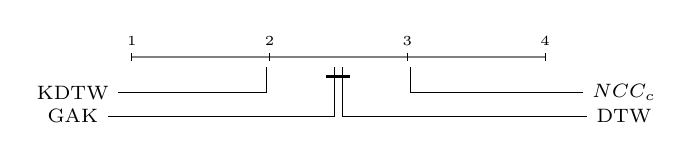
\begin{tikzpicture}[xscale=2]
\draw[gray, thick](00.8750, 0) -- (03.5000, 0);
\foreach \x in {00.8750,01.7500,02.6250,03.5000}\draw (\x cm,1.5pt) -- (\x cm, -1.5pt);
\node (Label) at (00.8750,0.2) {\tiny{1}};
\node (Label) at (01.7500,0.2) {\tiny{2}};
\node (Label) at (02.6250,0.2) {\tiny{3}};
\node (Label) at (03.5000,0.2) {\tiny{4}};
\draw[decorate,decoration={amplitude=.4mm,segment length=1.5mm,post length=0mm}, very thick, color = black](02.1104,-00.2500) -- ( 02.2611,-00.2500);
\node (Point) at (01.7325, 0){};  \node (Label) at (0.5,-00.4500){\scriptsize{KDTW}}; \draw (Point) |- (Label);
\node (Point) at (02.1604, 0){};  \node (Label) at (0.5,-00.7500){\scriptsize{GAK}}; \draw (Point) |- (Label);
\node (Point) at (02.6451, 0){};  \node (Label) at (4.0,-00.4500){\scriptsize{$NCC_c$}}; \draw (Point) |- (Label);
\node (Point) at (02.2111, 0){};  \node (Label) at (4.0,-00.7500){\scriptsize{DTW}}; \draw (Point) |- (Label);
\end{tikzpicture}
\vspace{-0.3cm}
\caption{\textcolor{black}{Ranking of kernel measures based on the average of their ranks across datasets, using supervised tuning.}}
\label{fig:kernel2}
\vspace{-0.3cm}
\end{figure}


\begin{figure} \centering 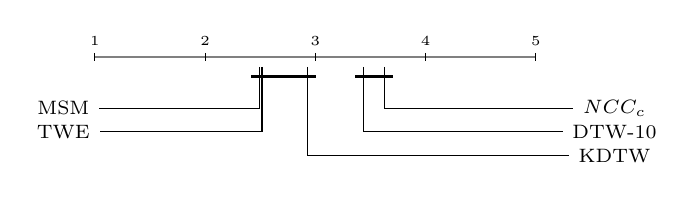
\begin{tikzpicture}[xscale=2]
\draw[gray, thick](00.7000, 0) -- (03.5000, 0);
\foreach \x in {00.7000,01.4000,02.1000,02.8000,03.5000}\draw (\x cm,1.5pt) -- (\x cm, -1.5pt);
\node (Label) at (00.7000,0.2) {\tiny{1}};
\node (Label) at (01.4000,0.2) {\tiny{2}};
\node (Label) at (02.1000,0.2) {\tiny{3}};
\node (Label) at (02.8000,0.2) {\tiny{4}};
\node (Label) at (03.5000,0.2) {\tiny{5}};
\draw[decorate,decoration={amplitude=.4mm,segment length=1.5mm,post length=0mm}, very thick, color = black](01.6944,-00.2500) -- ( 02.1010,-00.2500);
\draw[decorate,decoration={amplitude=.4mm,segment length=1.5mm,post length=0mm}, very thick, color = black](02.3538,-00.2500) -- ( 02.5903,-00.2500);
\node (Point) at (01.7444, 0){};  \node (Label) at (0.5,-00.6500){\scriptsize{MSM}}; \draw (Point) |- (Label);
\node (Point) at (01.7612, 0){};  \node (Label) at (0.5,-00.9500){\scriptsize{TWE}}; \draw (Point) |- (Label);
\node (Point) at (02.5403, 0){};  \node (Label) at (4.0,-00.6500){\scriptsize{$NCC_c$}}; \draw (Point) |- (Label);
\node (Point) at (02.4038, 0){};  \node (Label) at (4.0,-00.9500){\scriptsize{DTW-10}}; \draw (Point) |- (Label);
\node (Point) at (02.0510, 0){};  \node (Label) at (4.0,-01.2500){\scriptsize{KDTW}}; \draw (Point) |- (Label);
\end{tikzpicture}
\vspace{-0.3cm}
\caption{\textcolor{black}{Ranking of kernel measures based on the average of their ranks across datasets, using unsupervised tuning.}}
\label{fig:kernel3}
\vspace{-0.3cm}
\end{figure}

\section{Time-Series Embedding Measures}
\label{sec:embedded}
\textcolor{black}{Previously, we studied approaches that directly exploit a kernel function or a distance measure to compare time series. In this section, we study $4$ embedding measures, which are alternative approaches that employ a similarity measure only to construct new representations \cite{abanda2019review}. These representations are similarity-preserving as the comparison of two representations with ED approximates the comparison of the corresponding original time series with the employed similarity measure used to construct the representations.}

\textcolor{black}{We consider $4$ approaches to construct embedding measures (i.e., ED over learned representations). Specifically, we consider the Generic RepresentAtIon Learning (GRAIL) framework, which employs the SINK kernel \cite{paparrizos2019grail}, the Shift-invariant Dictionary Learning (SIDL) method, which preserves alignment between time series \cite{zheng2016efficient}, the Similarity Preserving Representation Learning method (SPIRAL), which employs DTW \cite{lei2017similarity}, and the Random Warping Series (RWS), which preserves the GAK kernel \cite{wu2018random}.}

\begin{table}[]
\setlength{\tabcolsep}{4.3pt}
\small
\centering
\begin{tabular}{|c|c|c|c|c|c|c|}
\hline
\textbf{\begin{tabular}[c]{@{}c@{}}Distance \\ Measure\end{tabular}} & \textbf{\begin{tabular}[c]{@{}c@{}}Parameter \\ Tuning\end{tabular}} & \textbf{\begin{tabular}[c]{@{}c@{}}Better\end{tabular}} & \textbf{\begin{tabular}[c]{@{}c@{}}Average \\ Accuracy\end{tabular}} & \textbf{\textgreater{}} & \textbf{=} & \textbf{\textless{}} \\ \hline
\begin{tabular}[c]{@{}c@{}}
GRAIL\end{tabular} &LOOCCV& \textcolor{BrickRed}{\ding{56}}&	0.7407 &56&8&64 \\ 


RWS &LOOCCV& \textcolor{NavyBlue}{\ding{74}}& 0.7128&45&3&80 \\ 

SPIRAL & - &  \textcolor{NavyBlue}{\ding{74}}& 0.6494&26&4&98 \\

SIDL &LOOCCV& \textcolor{NavyBlue}{\ding{74}}& 0.5759&12&1&115 \\ 


\hline
\textbf{NCC$_{c}$} & \textbf{-} & \textbf{-} & \textbf{0.7309} & \textbf{-} &	\textbf{-} & \textbf{-} \\ \hline
\end{tabular}
\caption{\textcolor{black}{Comparison of embedding measures. ``Better'' denotes that the distance measure outperforms the baseline with statistical significance. ``Average Accuracy'' shows the mean accuracy achieved across $128$ datasets. The last three columns indicate the datasets over which a measure is better (``>''), equal (``=''), or worse (``<'') than the baseline.}
}
\label{table:embedded}
\vspace{-0.3cm}
\end{table}


%\begin{figure} \centering \begin{tikzpicture}[xscale=2]
%\draw[gray, thick](00.7000, 0) -- (03.5000, 0);
%\foreach \x in {00.7000,01.4000,02.1000,02.8000,03.5000}\draw (\x cm,1.5pt) -- (\x cm, -1.5pt);
%\node (Label) at (00.7000,0.2) {\tiny{1}};
%\node (Label) at (01.4000,0.2) {\tiny{2}};
%\node (Label) at (02.1000,0.2) {\tiny{3}};
%\node (Label) at (02.8000,0.2) {\tiny{4}};
%\node (Label) at (03.5000,0.2) {\tiny{5}};
%\draw[decorate,decoration={amplitude=.4mm,segment length=1.5mm,post length=0mm}, very thick, color = black](01.6209,-00.2500) -- ( 01.9092,-00.2500);
%\draw[decorate,decoration={amplitude=.4mm,segment length=1.5mm,post length=0mm}, very thick, color = black](02.6681,-00.2500) -- ( 02.9949,-00.2500);
%\node (Point) at (01.3069, 0){};  \node (Label) at (0.5,-00.6500){\scriptsize{GRAIL}}; \draw (Point) |- (Label);
%\node (Point) at (01.6709, 0){};  \node (Label) at (0.5,-00.9500){\scriptsize{RWS}}; \draw (Point) |- (Label);
%\node (Point) at (02.9449, 0){};  \node (Label) at (4.0,-00.6500){\scriptsize{SIDL}}; \draw (Point) |- (Label);
%\node (Point) at (02.7181, 0){};  \node (Label) at (4.0,-00.9500){\scriptsize{SPIRAL}}; \draw (Point) |- (Label);
%\node (Point) at (01.8592, 0){};  \node (Label) at (4.0,-01.2500){\scriptsize{NCCc}}; \draw (Point) |- (Label);
%\end{tikzpicture}
%\vspace{-0.3cm}
%\caption{\textcolor{black}{Ranking of embedded measures based on the average of their ranks across datasets, using supervised tuning for their parameters.}}
%\label{fig:embedded3}
%\vspace{-0.3cm}
%\end{figure}

\newline \noindent \textbf{Evaluation of embedding measures: } \textcolor{black}{For all approaches, we follow \cite{paparrizos2019grail} and tune required parameters using the recommended  values  from  their  corresponding  papers. We construct representations of same length (100) for fairness. Table \ref{table:embedded} presents the results against NCC$_{c}$. We observe that GRAIL, is the only framework that constructs robust representations that when ED is used for comparison (under the 1-NN settings), it achieves similar performance to NCC$_{c}$, but without significant difference. All other embedding measures perform significantly worse (marked with \textcolor{NavyBlue}{\ding{74}}) and none of the embedding measures outperform DTW. We note, however, that embedding measures (as well as kernel methods), achieve much higher accuracy under different evaluation frameworks (e.g., with SVM classifiers), as shown in \cite{paparrizos2019grail}. We leave such extensive analysis for future work.}

\section{Accuracy-to-runtime Analysis}
\label{sec:overall}

\textcolor{black}{Until now, we performed an extensive evaluation of distance measures based on their accuracy results. However, it is also important to understand the cost associated with each one of these distance measures. In Figure \ref{fig:accuracyruntime}, we summarize the accuracy-to-runtime performance of the most prominent measures. The runtime performance includes only inference time (i.e., evaluation on the testing sets). We observe that ED, and all lock-step measures (omitted), are the fastest, but achieve relatively low accuracy (all these measures have $\mathcal{O}(m)$ runtime cost). NCC$_c$ and SINK, two methods that rely on the classic cross-correlation measure, provide a good trade-off between runtime and accuracy in comparison to ED (these measures have $\mathcal{O}(m \log m)$ runtime cost). We observe that all other elastic or kernel methods require substantially higher runtime cost to achieve comparable accuracy results to $NCC_c$ (these measures have $\mathcal{O}(m^2)$ runtime cost). We also observe that embedding measures show promise as they can be both efficient and accurate. We note that for elastic measures, the runtime cost can be substantially improved with the use of lower bounding measures (i.e., efficient measures to prune the expensive pairwise comparisons). To the best of our knowledge, for NCC$_c$ and the kernel methods, no lower bounding measures exist and, therefore, we leave such extensive runtime analysis for future work. Finally, Figure \ref{fig:error} suggests that with increasingly larger dataset sizes the classification error of ED may not always converge to the error of more accurate measures, at least not always with the same speed of convergence, which highlights the importance of considering measures other than ED (see Section \ref{sec:perceptions}). }


\begin{figure}[t]
	\vspace*{-0.2cm}
	\centering
	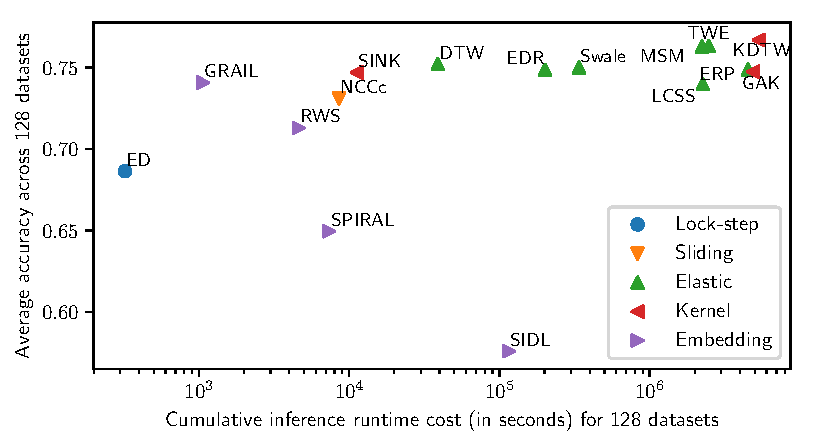
\includegraphics[height=4cm,width=8.2cm]{runtime-dis-log.pdf}
	\vspace*{-0.3cm}
	\caption{\textcolor{black}{Accuracy-to-runtime comparison.}}%
	\label{fig:accuracyruntime}%
	\vspace*{-0.3cm}
\end{figure}


\begin{figure}[t]
	%\vspace*{-0.2cm}
	\centering
	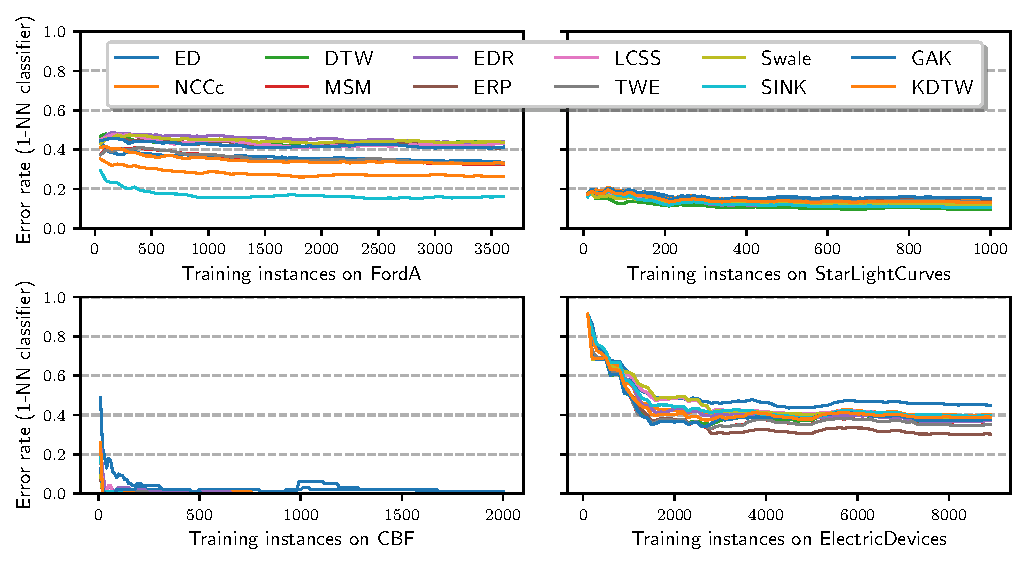
\includegraphics[height=4cm,width=8.2cm]{four-dataset-1nn22.pdf}
	\vspace*{-0.3cm}
	\caption{\textcolor{black}{Error rates with increasingly larger datasets.}}%
	\label{fig:error}%
	\vspace*{-0.3cm}
\end{figure}

%Our extensive experimental evaluation debunked four long-standing perceptions about time-series distance measures that, we believe, significantly alter the landscape of what is known about existing distance measures. In summary, we identified (i) normalization methods that in combination with various ---unknown until now--- distance measures lead to significant improvements in accuracy (e.g., Jaccard with MeanNorm and Emanon4 with MinMax distance measures); (ii) new lock-step measures that significantly outperform ED, the current state-of-the-art lock-step measure (e.g., Lorentzian distance); (iii) an omitted baseline, namely, the cross-correlation measure, that most of the highly popular elastic measures do not outperform; and (iv) new elastic measures, namely, MSM and TWE, that significantly outperform DTW, the current state-of-the-art elastic measure.


%\noindent \textbf{Better than elastic: } Elastic measures currently hold the title of the most accurate distance measures for time-series comparison. However, new categories of distance measures starting being explored (e.g., kernel functions and embedded measures \cite{abanda2019review}). It remains open if any of these types of measures can significantly outperform elastic measures. 

\section{Conclusion}
\label{sec:conclusions}

We presented a comprehensive evaluation to validate the performance of $71$ distance measures. Our study not only debunked four long-standing misconceptions in the time-series literature but also established new state-of-the-art results for lock-step, sliding, elastic, kernel, and embedding measures. Our findings prepare the ground to facilitate further development of distance measures with implications to virtually every task. With the new knowledge in place, several new challenges open that we hope to sparkle new research directions. For example, identifying more accurate normalizations will result in substantial improvement for many tasks. There is a lack of methods for unsupervised tuning of parameters. Finally, embedding measures might show the most promise considering their runtime-to-accuracy trade-off.
{\scriptsize  \newline \textbf{Acknowledgments: }
We thank the anonymous reviewers whose comments have greatly improved this manuscript. We also thank Themis Palpanas and Eamonn Keogh for useful discussions after acceptance. This research was supported in part by a Google  DAPA  Research  Award, gifts from NetApp, Cisco Systems, and Exelon Utilities, and an NSF Award CCF-1139158. Results presented in this paper were obtained using the Chameleon testbed supported by the National Science Foundation.}
%, but three categories of measures but, importantly, debunks four long-standing perceptions in the time-series literature that are concerned with the (i) normalization of time series; (ii) identification of the best measure per category; (iii) effect of omitted baselines in current measures; and (iv) detection of the best category of distance measures. Our findings prepare the ground to facilitate further development of distance measures with implications to every time-series task.


% ensure same length columns on last page (might need two sub-sequent latex runs)
\balance

\bibliographystyle{ACM-Reference-Format}
\bibliography{sample-bibliography}

\end{document}
